\documentclass[1p]{elsarticle_modified}
%\bibliographystyle{elsarticle-num}

%\usepackage[colorlinks]{hyperref}
%\usepackage{abbrmath_seonhwa} %\Abb, \Ascr, \Acal ,\Abf, \Afrak
\usepackage{amsfonts}
\usepackage{amssymb}
\usepackage{amsmath}
\usepackage{amsthm}
\usepackage{scalefnt}
\usepackage{amsbsy}
\usepackage{kotex}
\usepackage{caption}
\usepackage{subfig}
\usepackage{color}
\usepackage{graphicx}
\usepackage{xcolor} %% white, black, red, green, blue, cyan, magenta, yellow
\usepackage{float}
\usepackage{setspace}
\usepackage{hyperref}

\usepackage{tikz}
\usetikzlibrary{arrows}

\usepackage{multirow}
\usepackage{array} % fixed length table
\usepackage{hhline}

%%%%%%%%%%%%%%%%%%%%%
\makeatletter
\renewcommand*\env@matrix[1][\arraystretch]{%
	\edef\arraystretch{#1}%
	\hskip -\arraycolsep
	\let\@ifnextchar\new@ifnextchar
	\array{*\c@MaxMatrixCols c}}
\makeatother %https://tex.stackexchange.com/questions/14071/how-can-i-increase-the-line-spacing-in-a-matrix
%%%%%%%%%%%%%%%

\usepackage[normalem]{ulem}

\newcommand{\msout}[1]{\ifmmode\text{\sout{\ensuremath{#1}}}\else\sout{#1}\fi}
%SOURCE: \msout is \stkout macro in https://tex.stackexchange.com/questions/20609/strikeout-in-math-mode

\newcommand{\cancel}[1]{
	\ifmmode
	{\color{red}\msout{#1}}
	\else
	{\color{red}\sout{#1}}
	\fi
}

\newcommand{\add}[1]{
	{\color{blue}\uwave{#1}}
}

\newcommand{\replace}[2]{
	\ifmmode
	{\color{red}\msout{#1}}{\color{blue}\uwave{#2}}
	\else
	{\color{red}\sout{#1}}{\color{blue}\uwave{#2}}
	\fi
}

\newcommand{\Sol}{\mathcal{S}} %segment
\newcommand{\D}{D} %diagram
\newcommand{\A}{\mathcal{A}} %arc


%%%%%%%%%%%%%%%%%%%%%%%%%%%%%5 test

\def\sl{\operatorname{\textup{SL}}(2,\Cbb)}
\def\psl{\operatorname{\textup{PSL}}(2,\Cbb)}
\def\quan{\mkern 1mu \triangleright \mkern 1mu}

\theoremstyle{definition}
\newtheorem{thm}{Theorem}[section]
\newtheorem{prop}[thm]{Proposition}
\newtheorem{lem}[thm]{Lemma}
\newtheorem{ques}[thm]{Question}
\newtheorem{cor}[thm]{Corollary}
\newtheorem{defn}[thm]{Definition}
\newtheorem{exam}[thm]{Example}
\newtheorem{rmk}[thm]{Remark}
\newtheorem{alg}[thm]{Algorithm}

\newcommand{\I}{\sqrt{-1}}
\begin{document}

%\begin{frontmatter}
%
%\title{Boundary parabolic representations of knots up to 8 crossings}
%
%%% Group authors per affiliation:
%\author{Yunhi Cho} 
%\address{Department of Mathematics, University of Seoul, Seoul, Korea}
%\ead{yhcho@uos.ac.kr}
%
%
%\author{Seonhwa Kim} %\fnref{s_kim}}
%\address{Center for Geometry and Physics, Institute for Basic Science, Pohang, 37673, Korea}
%\ead{ryeona17@ibs.re.kr}
%
%\author{Hyuk Kim}
%\address{Department of Mathematical Sciences, Seoul National University, Seoul 08826, Korea}
%\ead{hyukkim@snu.ac.kr}
%
%\author{Seokbeom Yoon}
%\address{Department of Mathematical Sciences, Seoul National University, Seoul, 08826,  Korea}
%\ead{sbyoon15@snu.ac.kr}
%
%\begin{abstract}
%We find all boundary parabolic representation of knots up to 8 crossings.
%
%\end{abstract}
%\begin{keyword}
%    \MSC[2010] 57M25 
%\end{keyword}
%
%\end{frontmatter}

%\linenumbers
%\tableofcontents
%
\newcommand\colored[1]{\textcolor{white}{\rule[-0.35ex]{0.8em}{1.4ex}}\kern-0.8em\color{red} #1}%
%\newcommand\colored[1]{\textcolor{white}{ #1}\kern-2.17ex	\textcolor{white}{ #1}\kern-1.81ex	\textcolor{white}{ #1}\kern-2.15ex\color{red}#1	}

{\Large $\underline{11a_{350}~(K11a_{350})}$}

\setlength{\tabcolsep}{10pt}
\renewcommand{\arraystretch}{1.6}
\vspace{1cm}\begin{tabular}{m{100pt}>{\centering\arraybackslash}m{274pt}}
\multirow{5}{120pt}{
	\centering
	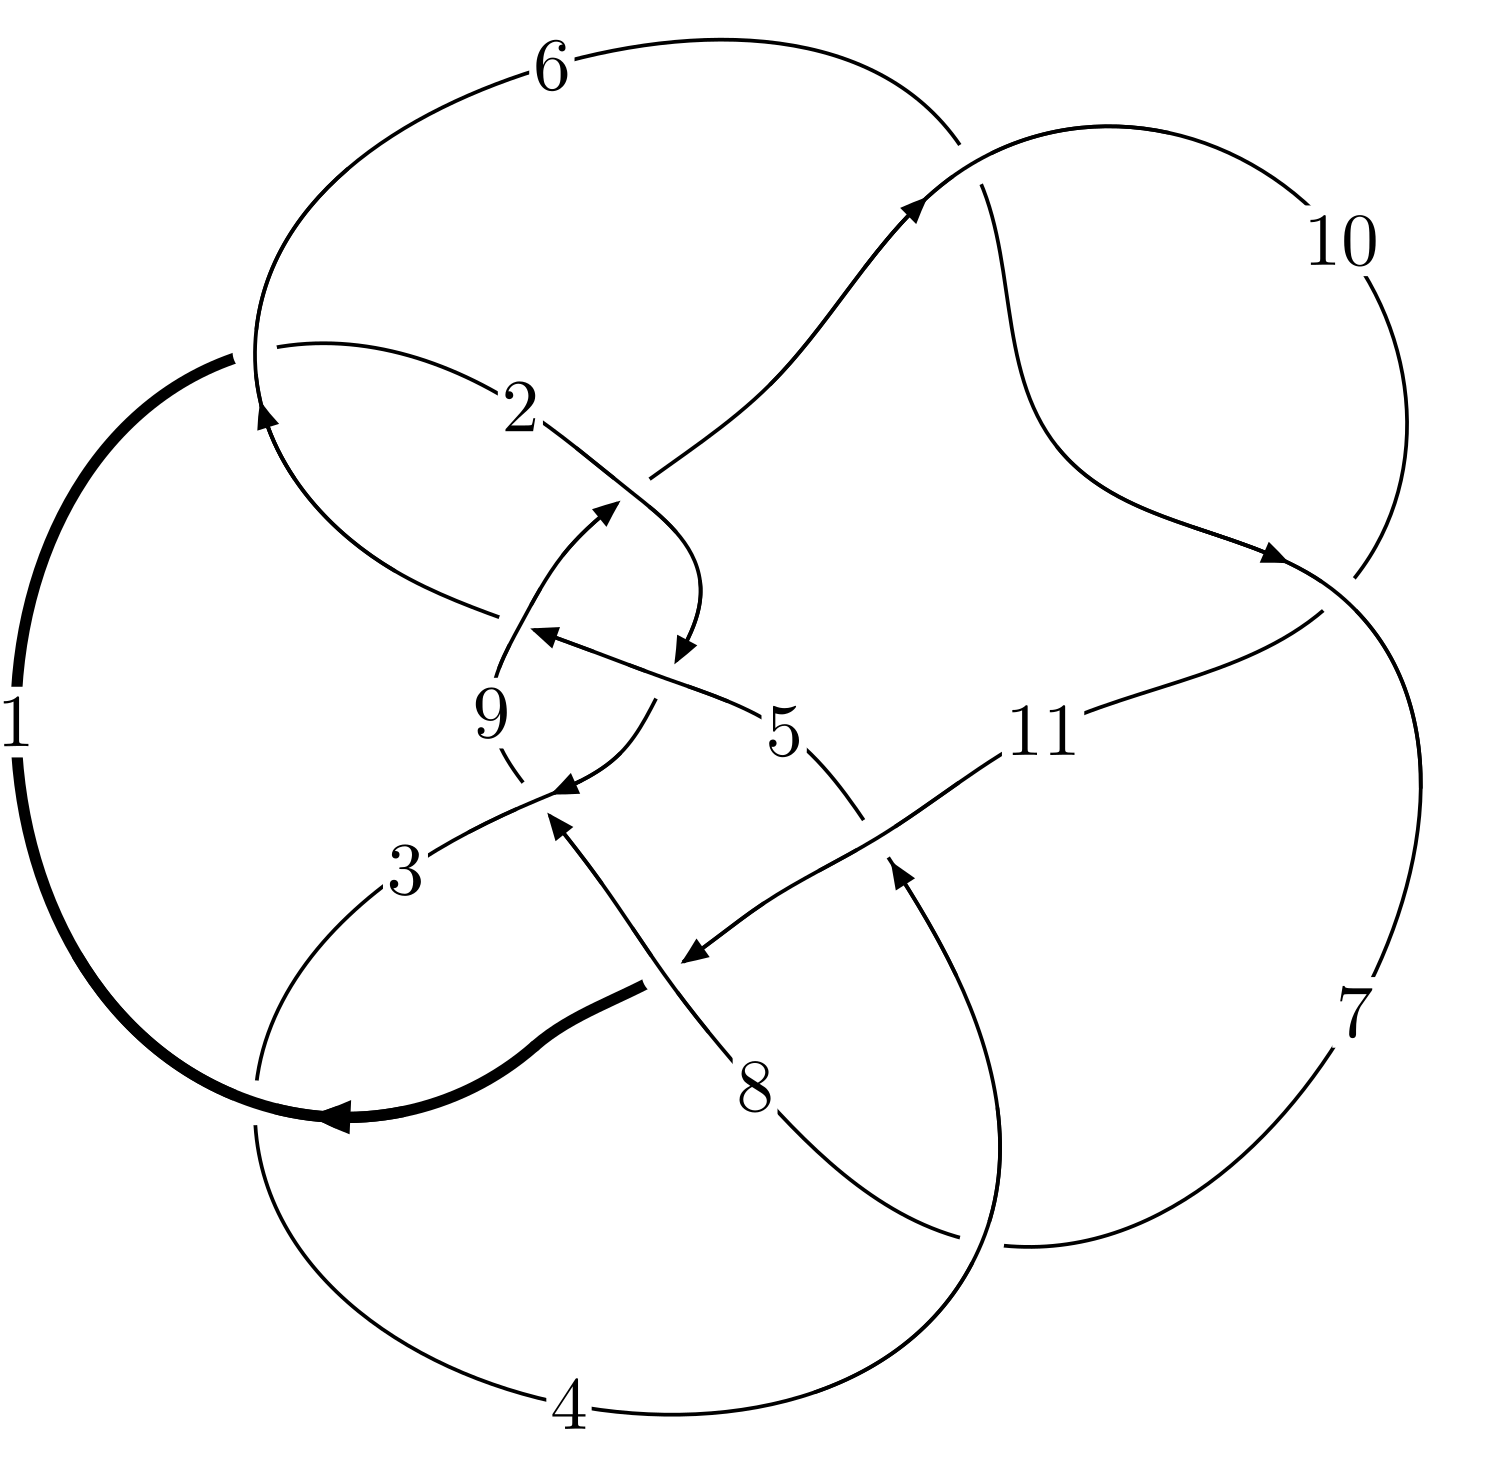
\includegraphics[width=112pt]{../../../GIT/diagram.site/Diagrams/png/599_11a_350.png}\\
\ \ \ A knot diagram\footnotemark}&
\allowdisplaybreaks
\textbf{Linearized knot diagam} \\
\cline{2-2}
 &
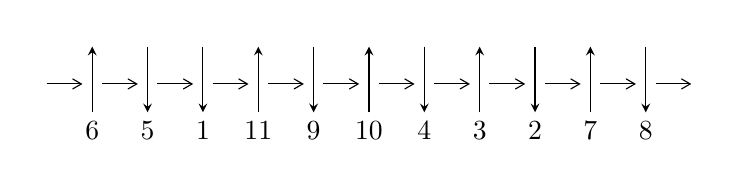
\begin{tikzpicture}[x=20pt, y=17pt]
	% nodes
	\node (C0) at (0, 0) {};
	\node (C1) at (1, 0) {};
	\node (C1U) at (1, +1) {};
	\node (C1D) at (1, -1) {6};

	\node (C2) at (2, 0) {};
	\node (C2U) at (2, +1) {};
	\node (C2D) at (2, -1) {5};

	\node (C3) at (3, 0) {};
	\node (C3U) at (3, +1) {};
	\node (C3D) at (3, -1) {1};

	\node (C4) at (4, 0) {};
	\node (C4U) at (4, +1) {};
	\node (C4D) at (4, -1) {11};

	\node (C5) at (5, 0) {};
	\node (C5U) at (5, +1) {};
	\node (C5D) at (5, -1) {9};

	\node (C6) at (6, 0) {};
	\node (C6U) at (6, +1) {};
	\node (C6D) at (6, -1) {10};

	\node (C7) at (7, 0) {};
	\node (C7U) at (7, +1) {};
	\node (C7D) at (7, -1) {4};

	\node (C8) at (8, 0) {};
	\node (C8U) at (8, +1) {};
	\node (C8D) at (8, -1) {3};

	\node (C9) at (9, 0) {};
	\node (C9U) at (9, +1) {};
	\node (C9D) at (9, -1) {2};

	\node (C10) at (10, 0) {};
	\node (C10U) at (10, +1) {};
	\node (C10D) at (10, -1) {7};

	\node (C11) at (11, 0) {};
	\node (C11U) at (11, +1) {};
	\node (C11D) at (11, -1) {8};
	\node (C12) at (12, 0) {};

	% arrows
	\draw[->,>={angle 60}]
	(C0) edge (C1) (C1) edge (C2) (C2) edge (C3) (C3) edge (C4) (C4) edge (C5) (C5) edge (C6) (C6) edge (C7) (C7) edge (C8) (C8) edge (C9) (C9) edge (C10) (C10) edge (C11) (C11) edge (C12) ;	\draw[->,>=stealth]
	(C1D) edge (C1U) (C2U) edge (C2D) (C3U) edge (C3D) (C4D) edge (C4U) (C5U) edge (C5D) (C6D) edge (C6U) (C7U) edge (C7D) (C8D) edge (C8U) (C9U) edge (C9D) (C10D) edge (C10U) (C11U) edge (C11D) ;
	\end{tikzpicture} \\
\hhline{~~} \\& 
\textbf{Solving Sequence} \\ \cline{2-2} 
 &
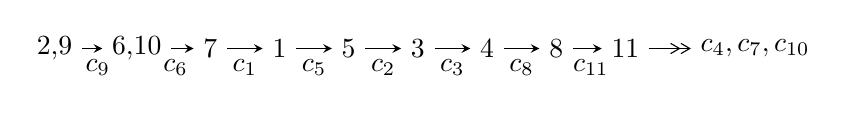
\begin{tikzpicture}[x=25pt, y=7pt]
	% node
	\node (A0) at (-1/8, 0) {2,9};
	\node (A1) at (17/16, 0) {6,10};
	\node (A2) at (17/8, 0) {7};
	\node (A3) at (25/8, 0) {1};
	\node (A4) at (33/8, 0) {5};
	\node (A5) at (41/8, 0) {3};
	\node (A6) at (49/8, 0) {4};
	\node (A7) at (57/8, 0) {8};
	\node (A8) at (65/8, 0) {11};
	\node (C1) at (1/2, -1) {$c_{9}$};
	\node (C2) at (13/8, -1) {$c_{6}$};
	\node (C3) at (21/8, -1) {$c_{1}$};
	\node (C4) at (29/8, -1) {$c_{5}$};
	\node (C5) at (37/8, -1) {$c_{2}$};
	\node (C6) at (45/8, -1) {$c_{3}$};
	\node (C7) at (53/8, -1) {$c_{8}$};
	\node (C8) at (61/8, -1) {$c_{11}$};
	\node (A9) at (10, 0) {$c_{4},c_{7},c_{10}$};

	% edge
	\draw[->,>=stealth]	
	(A0) edge (A1) (A1) edge (A2) (A2) edge (A3) (A3) edge (A4) (A4) edge (A5) (A5) edge (A6) (A6) edge (A7) (A7) edge (A8) ;
	\draw[->>,>={angle 60}]	
	(A8) edge (A9);
\end{tikzpicture} \\ 

\end{tabular} \\

\footnotetext{
The image of knot diagram is generated by the software ``\textbf{Draw programme}" developed by Andrew Bartholomew(\url{http://www.layer8.co.uk/maths/draw/index.htm\#Running-draw}), where we modified some parts for our purpose(\url{https://github.com/CATsTAILs/LinksPainter}).
}\phantom \\ \newline 
\centering \textbf{Ideals for irreducible components\footnotemark of $X_{\text{par}}$} 
 
\begin{align*}
I^u_{1}&=\langle 
-3.21880\times10^{22} u^{23}-1.45306\times10^{23} u^{22}+\cdots+1.84096\times10^{22} b-1.77351\times10^{21},\\
\phantom{I^u_{1}}&\phantom{= \langle  }1.69641\times10^{22} u^{23}+1.16788\times10^{23} u^{22}+\cdots+1.84096\times10^{22} a+9.02386\times10^{22},\;u^{24}+5 u^{23}+\cdots+5 u+1\rangle \\
I^u_{2}&=\langle 
-6.31384\times10^{394} u^{89}+6.92476\times10^{394} u^{88}+\cdots+7.51178\times10^{396} b-8.98383\times10^{397},\\
\phantom{I^u_{2}}&\phantom{= \langle  }-1.55103\times10^{397} u^{89}-2.32083\times10^{398} u^{88}+\cdots+5.23571\times10^{399} a+6.11690\times10^{401},\\
\phantom{I^u_{2}}&\phantom{= \langle  }u^{90}+13 u^{88}+\cdots-2331 u-697\rangle \\
I^u_{3}&=\langle 
596388417531502 u^{19}-535727113968989 u^{18}+\cdots+1506447924749558 b-1004384011943253,\\
\phantom{I^u_{3}}&\phantom{= \langle  }1534485576412749 u^{19}+1924336217084222 u^{18}+\cdots+1506447924749558 a+5029781266974281,\\
\phantom{I^u_{3}}&\phantom{= \langle  }u^{20}+12 u^{18}+\cdots+2 u+1\rangle \\
I^u_{4}&=\langle 
u^3+u^2+b- u-1,\;- u^3- u^2+a+2 u+1,\;u^4+u^3- u^2- u-1\rangle \\
I^u_{5}&=\langle 
b+u,\;a- u-1,\;u^2+u+1\rangle \\
\\
\end{align*}
\raggedright * 5 irreducible components of $\dim_{\mathbb{C}}=0$, with total 140 representations.\\
\footnotetext{All coefficients of polynomials are rational numbers. But the coefficients are sometimes approximated in decimal forms when there is not enough margin.}
\newpage
\renewcommand{\arraystretch}{1}
\centering \section*{I. $I^u_{1}= \langle -3.22\times10^{22} u^{23}-1.45\times10^{23} u^{22}+\cdots+1.84\times10^{22} b-1.77\times10^{21},\;1.70\times10^{22} u^{23}+1.17\times10^{23} u^{22}+\cdots+1.84\times10^{22} a+9.02\times10^{22},\;u^{24}+5 u^{23}+\cdots+5 u+1 \rangle$}
\flushleft \textbf{(i) Arc colorings}\\
\begin{tabular}{m{7pt} m{180pt} m{7pt} m{180pt} }
\flushright $a_{2}=$&$\begin{pmatrix}0\\u\end{pmatrix}$ \\
\flushright $a_{9}=$&$\begin{pmatrix}1\\0\end{pmatrix}$ \\
\flushright $a_{6}=$&$\begin{pmatrix}-0.921482 u^{23}-6.34386 u^{22}+\cdots-16.1753 u-4.90172\\1.74844 u^{23}+7.89293 u^{22}+\cdots+5.65599 u+0.0963361\end{pmatrix}$ \\
\flushright $a_{10}=$&$\begin{pmatrix}1\\u^2\end{pmatrix}$ \\
\flushright $a_{7}=$&$\begin{pmatrix}-0.803405 u^{23}-6.36897 u^{22}+\cdots-20.1230 u-6.54183\\1.95379 u^{23}+9.10729 u^{22}+\cdots+8.61541 u+0.711836\end{pmatrix}$ \\
\flushright $a_{1}=$&$\begin{pmatrix}5.52017 u^{23}+30.5886 u^{22}+\cdots+53.7538 u+10.3116\\-4.04248 u^{23}-19.7310 u^{22}+\cdots-22.7797 u-4.62275\end{pmatrix}$ \\
\flushright $a_{5}=$&$\begin{pmatrix}0.826954 u^{23}+1.54907 u^{22}+\cdots-10.5193 u-4.80538\\1.74844 u^{23}+7.89293 u^{22}+\cdots+5.65599 u+0.0963361\end{pmatrix}$ \\
\flushright $a_{3}=$&$\begin{pmatrix}0.624051 u^{23}+5.42049 u^{22}+\cdots+12.4325 u+0.988234\\-0.853640 u^{23}-5.43714 u^{22}+\cdots-16.5416 u-4.70063\end{pmatrix}$ \\
\flushright $a_{4}=$&$\begin{pmatrix}-9.64576 u^{23}-47.9185 u^{22}+\cdots-65.9753 u-12.2608\\1.74443 u^{23}+8.33782 u^{22}+\cdots+5.56945 u+0.493106\end{pmatrix}$ \\
\flushright $a_{8}=$&$\begin{pmatrix}-0.493106 u^{23}-0.721096 u^{22}+\cdots+15.8450 u+3.10392\\1.56945 u^{23}+6.25870 u^{22}+\cdots+0.386352 u-1.03260\end{pmatrix}$ \\
\flushright $a_{11}=$&$\begin{pmatrix}2.20692 u^{23}+13.4346 u^{22}+\cdots+38.8975 u+9.36897\\-1.36287 u^{23}-5.75236 u^{22}+\cdots+2.19259 u+1.11471\end{pmatrix}$\\ \flushright $a_{11}=$&$\begin{pmatrix}2.20692 u^{23}+13.4346 u^{22}+\cdots+38.8975 u+9.36897\\-1.36287 u^{23}-5.75236 u^{22}+\cdots+2.19259 u+1.11471\end{pmatrix}$\\&\end{tabular}
\flushleft \textbf{(ii) Obstruction class $= -1$}\\~\\
\flushleft \textbf{(iii) Cusp Shapes $= \frac{504150061088705768350224}{18409584491066375925047} u^{23}+\frac{2533975755434351329384291}{18409584491066375925047} u^{22}+\cdots+\frac{2937396997691488250591708}{18409584491066375925047} u+\frac{478043081351450205457199}{18409584491066375925047}$}\\~\\
\newpage\renewcommand{\arraystretch}{1}
\flushleft \textbf{(iv) u-Polynomials at the component}\newline \\
\begin{tabular}{m{50pt}|m{274pt}}
Crossings & \hspace{64pt}u-Polynomials at each crossing \\
\hline $$\begin{aligned}c_{1},c_{4}\end{aligned}$$&$\begin{aligned}
&u^{24}+5 u^{23}+\cdots+8 u+1
\end{aligned}$\\
\hline $$\begin{aligned}c_{2},c_{3}\end{aligned}$$&$\begin{aligned}
&u^{24}+3 u^{23}+\cdots+3 u+1
\end{aligned}$\\
\hline $$\begin{aligned}c_{5},c_{11}\end{aligned}$$&$\begin{aligned}
&u^{24}+u^{23}+\cdots+7 u+1
\end{aligned}$\\
\hline $$\begin{aligned}c_{6},c_{10}\end{aligned}$$&$\begin{aligned}
&u^{24}-2 u^{23}+\cdots-106 u+36
\end{aligned}$\\
\hline $$\begin{aligned}c_{7},c_{9}\end{aligned}$$&$\begin{aligned}
&u^{24}-5 u^{23}+\cdots-5 u+1
\end{aligned}$\\
\hline $$\begin{aligned}c_{8}\end{aligned}$$&$\begin{aligned}
&u^{24}- u^{23}+\cdots+320 u+64
\end{aligned}$\\
\hline
\end{tabular}\\~\\
\newpage\renewcommand{\arraystretch}{1}
\flushleft \textbf{(v) Riley Polynomials at the component}\newline \\
\begin{tabular}{m{50pt}|m{274pt}}
Crossings & \hspace{64pt}Riley Polynomials at each crossing \\
\hline $$\begin{aligned}c_{1},c_{4}\end{aligned}$$&$\begin{aligned}
&y^{24}-7 y^{23}+\cdots-6 y+1
\end{aligned}$\\
\hline $$\begin{aligned}c_{2},c_{3}\end{aligned}$$&$\begin{aligned}
&y^{24}+3 y^{23}+\cdots+27 y+1
\end{aligned}$\\
\hline $$\begin{aligned}c_{5},c_{11}\end{aligned}$$&$\begin{aligned}
&y^{24}+7 y^{23}+\cdots-29 y+1
\end{aligned}$\\
\hline $$\begin{aligned}c_{6},c_{10}\end{aligned}$$&$\begin{aligned}
&y^{24}-12 y^{23}+\cdots+9860 y+1296
\end{aligned}$\\
\hline $$\begin{aligned}c_{7},c_{9}\end{aligned}$$&$\begin{aligned}
&y^{24}-21 y^{23}+\cdots-5 y+1
\end{aligned}$\\
\hline $$\begin{aligned}c_{8}\end{aligned}$$&$\begin{aligned}
&y^{24}-23 y^{23}+\cdots+30720 y+4096
\end{aligned}$\\
\hline
\end{tabular}\\~\\
\newpage\flushleft \textbf{(vi) Complex Volumes and Cusp Shapes}
$$\begin{array}{c|c|c}  
\text{Solutions to }I^u_{1}& \I (\text{vol} + \sqrt{-1}CS) & \text{Cusp shape}\\
 \hline 
\begin{aligned}
u &= \phantom{-}0.948562 + 0.118544 I \\
a &= \phantom{-}0.386832 - 0.880975 I \\
b &= \phantom{-}0.589066 - 0.233963 I\end{aligned}
 & -2.99609 + 1.94907 I & -10.80827 - 2.58369 I \\ \hline\begin{aligned}
u &= \phantom{-}0.948562 - 0.118544 I \\
a &= \phantom{-}0.386832 + 0.880975 I \\
b &= \phantom{-}0.589066 + 0.233963 I\end{aligned}
 & -2.99609 - 1.94907 I & -10.80827 + 2.58369 I \\ \hline\begin{aligned}
u &= -0.397178 + 0.844071 I \\
a &= -0.65338 + 1.54955 I \\
b &= \phantom{-}0.017160 - 0.636778 I\end{aligned}
 & \phantom{-}5.31187 + 3.98651 I & \phantom{-}5.66668 - 8.11376 I \\ \hline\begin{aligned}
u &= -0.397178 - 0.844071 I \\
a &= -0.65338 - 1.54955 I \\
b &= \phantom{-}0.017160 + 0.636778 I\end{aligned}
 & \phantom{-}5.31187 - 3.98651 I & \phantom{-}5.66668 + 8.11376 I \\ \hline\begin{aligned}
u &= -0.897247 + 0.630246 I \\
a &= -0.175373 - 0.678747 I \\
b &= -0.458367 + 1.128800 I\end{aligned}
 & \phantom{-}1.59590 + 4.68195 I & \phantom{-}5.09129 - 10.67393 I \\ \hline\begin{aligned}
u &= -0.897247 - 0.630246 I \\
a &= -0.175373 + 0.678747 I \\
b &= -0.458367 - 1.128800 I\end{aligned}
 & \phantom{-}1.59590 - 4.68195 I & \phantom{-}5.09129 + 10.67393 I \\ \hline\begin{aligned}
u &= \phantom{-}0.669369 + 0.399651 I \\
a &= \phantom{-}0.199150 + 0.717971 I \\
b &= -1.22208 - 1.31312 I\end{aligned}
 & -0.94261 - 4.71787 I & -11.6555 + 14.8007 I \\ \hline\begin{aligned}
u &= \phantom{-}0.669369 - 0.399651 I \\
a &= \phantom{-}0.199150 - 0.717971 I \\
b &= -1.22208 + 1.31312 I\end{aligned}
 & -0.94261 + 4.71787 I & -11.6555 - 14.8007 I \\ \hline\begin{aligned}
u &= -0.275157 + 0.682551 I \\
a &= -0.34003 - 1.57031 I \\
b &= \phantom{-}1.02362 + 1.39590 I\end{aligned}
 & \phantom{-}5.80334 + 2.74033 I & \phantom{-}15.5158 - 11.8363 I \\ \hline\begin{aligned}
u &= -0.275157 - 0.682551 I \\
a &= -0.34003 + 1.57031 I \\
b &= \phantom{-}1.02362 - 1.39590 I\end{aligned}
 & \phantom{-}5.80334 - 2.74033 I & \phantom{-}15.5158 + 11.8363 I\\
 \hline 
 \end{array}$$\newpage$$\begin{array}{c|c|c}  
\text{Solutions to }I^u_{1}& \I (\text{vol} + \sqrt{-1}CS) & \text{Cusp shape}\\
 \hline 
\begin{aligned}
u &= -0.284422 + 0.660333 I \\
a &= -0.05560 - 2.91538 I \\
b &= \phantom{-}0.124798 + 1.311920 I\end{aligned}
 & \phantom{-}5.07438 + 1.59386 I & \phantom{-}2.13582 - 1.10254 I \\ \hline\begin{aligned}
u &= -0.284422 - 0.660333 I \\
a &= -0.05560 + 2.91538 I \\
b &= \phantom{-}0.124798 - 1.311920 I\end{aligned}
 & \phantom{-}5.07438 - 1.59386 I & \phantom{-}2.13582 + 1.10254 I \\ \hline\begin{aligned}
u &= -0.913544 + 0.934068 I \\
a &= -0.137387 + 0.975627 I \\
b &= \phantom{-}1.23496 - 1.04677 I\end{aligned}
 & -2.20266 + 13.23270 I & -2.28061 - 10.36959 I \\ \hline\begin{aligned}
u &= -0.913544 - 0.934068 I \\
a &= -0.137387 - 0.975627 I \\
b &= \phantom{-}1.23496 + 1.04677 I\end{aligned}
 & -2.20266 - 13.23270 I & -2.28061 + 10.36959 I \\ \hline\begin{aligned}
u &= \phantom{-}0.219244 + 0.655965 I \\
a &= \phantom{-}0.641636 + 0.616523 I \\
b &= -0.138317 - 0.535445 I\end{aligned}
 & \phantom{-}0.112664 - 1.342820 I & \phantom{-}0.96375 + 5.78549 I \\ \hline\begin{aligned}
u &= \phantom{-}0.219244 - 0.655965 I \\
a &= \phantom{-}0.641636 - 0.616523 I \\
b &= -0.138317 + 0.535445 I\end{aligned}
 & \phantom{-}0.112664 + 1.342820 I & \phantom{-}0.96375 - 5.78549 I \\ \hline\begin{aligned}
u &= \phantom{-}0.95916 + 1.28491 I \\
a &= \phantom{-}0.109942 + 1.076420 I \\
b &= -1.19384 - 1.00053 I\end{aligned}
 & \phantom{-}3.9513 - 19.3243 I & \phantom{-}0.92200 + 10.02171 I \\ \hline\begin{aligned}
u &= \phantom{-}0.95916 - 1.28491 I \\
a &= \phantom{-}0.109942 - 1.076420 I \\
b &= -1.19384 + 1.00053 I\end{aligned}
 & \phantom{-}3.9513 + 19.3243 I & \phantom{-}0.92200 - 10.02171 I \\ \hline\begin{aligned}
u &= -0.315740 + 0.142853 I \\
a &= -1.62304 + 1.34024 I \\
b &= -0.873029 + 0.698246 I\end{aligned}
 & \phantom{-}0.03065 + 2.94504 I & -0.62404 - 2.53282 I \\ \hline\begin{aligned}
u &= -0.315740 - 0.142853 I \\
a &= -1.62304 - 1.34024 I \\
b &= -0.873029 - 0.698246 I\end{aligned}
 & \phantom{-}0.03065 - 2.94504 I & -0.62404 + 2.53282 I\\
 \hline 
 \end{array}$$\newpage$$\begin{array}{c|c|c}  
\text{Solutions to }I^u_{1}& \I (\text{vol} + \sqrt{-1}CS) & \text{Cusp shape}\\
 \hline 
\begin{aligned}
u &= \phantom{-}0.99393 + 1.39275 I \\
a &= -0.078356 - 0.752209 I \\
b &= \phantom{-}0.690199 + 0.960956 I\end{aligned}
 & \phantom{-}7.26188 - 10.39510 I & \phantom{-}4.97109 + 9.26898 I \\ \hline\begin{aligned}
u &= \phantom{-}0.99393 - 1.39275 I \\
a &= -0.078356 + 0.752209 I \\
b &= \phantom{-}0.690199 - 0.960956 I\end{aligned}
 & \phantom{-}7.26188 + 10.39510 I & \phantom{-}4.97109 - 9.26898 I \\ \hline\begin{aligned}
u &= -1.80800\phantom{ +0.000000I} \\
a &= -0.491944\phantom{ +0.000000I} \\
b &= -0.412432\phantom{ +0.000000I}\end{aligned}
 & \phantom{-}0.0704593\phantom{ +0.000000I} & \phantom{-}10.7550\phantom{ +0.000000I} \\ \hline\begin{aligned}
u &= -4.60596\phantom{ +0.000000I} \\
a &= -0.0568603\phantom{ +0.000000I} \\
b &= -0.175899\phantom{ +0.000000I}\end{aligned}
 & -0.0136435\phantom{ +0.000000I} & \phantom{-0.000000 } 0\\
 \hline 
 \end{array}$$\newpage\newpage\renewcommand{\arraystretch}{1}
\centering \section*{II. $I^u_{2}= \langle -6.31\times10^{394} u^{89}+6.92\times10^{394} u^{88}+\cdots+7.51\times10^{396} b-8.98\times10^{397},\;-1.55\times10^{397} u^{89}-2.32\times10^{398} u^{88}+\cdots+5.24\times10^{399} a+6.12\times10^{401},\;u^{90}+13 u^{88}+\cdots-2331 u-697 \rangle$}
\flushleft \textbf{(i) Arc colorings}\\
\begin{tabular}{m{7pt} m{180pt} m{7pt} m{180pt} }
\flushright $a_{2}=$&$\begin{pmatrix}0\\u\end{pmatrix}$ \\
\flushright $a_{9}=$&$\begin{pmatrix}1\\0\end{pmatrix}$ \\
\flushright $a_{6}=$&$\begin{pmatrix}0.00296240 u^{89}+0.0443270 u^{88}+\cdots-438.837 u-116.830\\0.00840525 u^{89}-0.00921854 u^{88}+\cdots+35.0495 u+11.9597\end{pmatrix}$ \\
\flushright $a_{10}=$&$\begin{pmatrix}1\\u^2\end{pmatrix}$ \\
\flushright $a_{7}=$&$\begin{pmatrix}0.00615108 u^{89}+0.0463311 u^{88}+\cdots-509.179 u-135.767\\0.00721730 u^{89}-0.00830298 u^{88}+\cdots+41.9437 u+13.3565\end{pmatrix}$ \\
\flushright $a_{1}=$&$\begin{pmatrix}-0.0981362 u^{89}+0.00893073 u^{88}+\cdots-111.972 u-57.6678\\-0.00924215 u^{89}-0.00377916 u^{88}+\cdots+55.6357 u+10.3743\end{pmatrix}$ \\
\flushright $a_{5}=$&$\begin{pmatrix}0.0113676 u^{89}+0.0351084 u^{88}+\cdots-403.788 u-104.871\\0.00840525 u^{89}-0.00921854 u^{88}+\cdots+35.0495 u+11.9597\end{pmatrix}$ \\
\flushright $a_{3}=$&$\begin{pmatrix}-0.0987547 u^{89}+0.00556089 u^{88}+\cdots-75.5358 u-48.4670\\0.00862368 u^{89}+0.000409326 u^{88}+\cdots-17.1997 u-1.17357\end{pmatrix}$ \\
\flushright $a_{4}=$&$\begin{pmatrix}0.0318351 u^{89}+0.0633408 u^{88}+\cdots-419.152 u-85.0975\\0.00355555 u^{89}+0.00998720 u^{88}+\cdots-106.546 u-27.9283\end{pmatrix}$ \\
\flushright $a_{8}=$&$\begin{pmatrix}0.00442432 u^{89}-0.0678970 u^{88}+\cdots+531.689 u+122.167\\-0.0153682 u^{89}+0.0121057 u^{88}+\cdots-37.2591 u-23.9882\end{pmatrix}$ \\
\flushright $a_{11}=$&$\begin{pmatrix}0.00232107 u^{89}-0.0476243 u^{88}+\cdots+401.540 u+95.0377\\-0.0139733 u^{89}+0.0135534 u^{88}+\cdots-50.8930 u-27.4980\end{pmatrix}$\\ \flushright $a_{11}=$&$\begin{pmatrix}0.00232107 u^{89}-0.0476243 u^{88}+\cdots+401.540 u+95.0377\\-0.0139733 u^{89}+0.0135534 u^{88}+\cdots-50.8930 u-27.4980\end{pmatrix}$\\&\end{tabular}
\flushleft \textbf{(ii) Obstruction class $= -1$}\\~\\
\flushleft \textbf{(iii) Cusp Shapes $= -0.0316762 u^{89}-0.0348001 u^{88}+\cdots+220.805 u+45.4124$}\\~\\
\newpage\renewcommand{\arraystretch}{1}
\flushleft \textbf{(iv) u-Polynomials at the component}\newline \\
\begin{tabular}{m{50pt}|m{274pt}}
Crossings & \hspace{64pt}u-Polynomials at each crossing \\
\hline $$\begin{aligned}c_{1},c_{4}\end{aligned}$$&$\begin{aligned}
&u^{90}-4 u^{89}+\cdots-679 u-263
\end{aligned}$\\
\hline $$\begin{aligned}c_{2},c_{3}\end{aligned}$$&$\begin{aligned}
&u^{90}- u^{89}+\cdots-675 u+103
\end{aligned}$\\
\hline $$\begin{aligned}c_{5},c_{11}\end{aligned}$$&$\begin{aligned}
&u^{90}-8 u^{88}+\cdots-22 u-1
\end{aligned}$\\
\hline $$\begin{aligned}c_{6},c_{10}\end{aligned}$$&$\begin{aligned}
&(u^{45}-20 u^{43}+\cdots+189 u+108)^{2}
\end{aligned}$\\
\hline $$\begin{aligned}c_{7},c_{9}\end{aligned}$$&$\begin{aligned}
&u^{90}+13 u^{88}+\cdots+2331 u-697
\end{aligned}$\\
\hline $$\begin{aligned}c_{8}\end{aligned}$$&$\begin{aligned}
&(u^{45}-2 u^{44}+\cdots-45 u-9)^{2}
\end{aligned}$\\
\hline
\end{tabular}\\~\\
\newpage\renewcommand{\arraystretch}{1}
\flushleft \textbf{(v) Riley Polynomials at the component}\newline \\
\begin{tabular}{m{50pt}|m{274pt}}
Crossings & \hspace{64pt}Riley Polynomials at each crossing \\
\hline $$\begin{aligned}c_{1},c_{4}\end{aligned}$$&$\begin{aligned}
&y^{90}-20 y^{89}+\cdots-4190907 y+69169
\end{aligned}$\\
\hline $$\begin{aligned}c_{2},c_{3}\end{aligned}$$&$\begin{aligned}
&y^{90}-7 y^{89}+\cdots+296069 y+10609
\end{aligned}$\\
\hline $$\begin{aligned}c_{5},c_{11}\end{aligned}$$&$\begin{aligned}
&y^{90}-16 y^{89}+\cdots-90 y+1
\end{aligned}$\\
\hline $$\begin{aligned}c_{6},c_{10}\end{aligned}$$&$\begin{aligned}
&(y^{45}-40 y^{44}+\cdots-36207 y-11664)^{2}
\end{aligned}$\\
\hline $$\begin{aligned}c_{7},c_{9}\end{aligned}$$&$\begin{aligned}
&y^{90}+26 y^{89}+\cdots+21978055 y+485809
\end{aligned}$\\
\hline $$\begin{aligned}c_{8}\end{aligned}$$&$\begin{aligned}
&(y^{45}+20 y^{44}+\cdots+2871 y-81)^{2}
\end{aligned}$\\
\hline
\end{tabular}\\~\\
\newpage\flushleft \textbf{(vi) Complex Volumes and Cusp Shapes}
$$\begin{array}{c|c|c}  
\text{Solutions to }I^u_{2}& \I (\text{vol} + \sqrt{-1}CS) & \text{Cusp shape}\\
 \hline 
\begin{aligned}
u &= \phantom{-}0.650238 + 0.770616 I \\
a &= \phantom{-}0.756665 + 0.325666 I \\
b &= -0.157441 + 0.051744 I\end{aligned}
 & \phantom{-}0.40566 - 1.48274 I & \phantom{-0.000000 } 0 \\ \hline\begin{aligned}
u &= \phantom{-}0.650238 - 0.770616 I \\
a &= \phantom{-}0.756665 - 0.325666 I \\
b &= -0.157441 - 0.051744 I\end{aligned}
 & \phantom{-}0.40566 + 1.48274 I & \phantom{-0.000000 } 0 \\ \hline\begin{aligned}
u &= \phantom{-}0.408621 + 0.900284 I \\
a &= \phantom{-}0.240008 + 0.792608 I \\
b &= -0.439265 - 0.984349 I\end{aligned}
 & \phantom{-}0.40566 - 1.48274 I & \phantom{-0.000000 } 0 \\ \hline\begin{aligned}
u &= \phantom{-}0.408621 - 0.900284 I \\
a &= \phantom{-}0.240008 - 0.792608 I \\
b &= -0.439265 + 0.984349 I\end{aligned}
 & \phantom{-}0.40566 + 1.48274 I & \phantom{-0.000000 } 0 \\ \hline\begin{aligned}
u &= \phantom{-}0.167555 + 0.950964 I \\
a &= \phantom{-}0.199750 + 0.931839 I \\
b &= \phantom{-}0.748689 - 1.189060 I\end{aligned}
 & \phantom{-}2.94180 - 3.09675 I & \phantom{-0.000000 } 0 \\ \hline\begin{aligned}
u &= \phantom{-}0.167555 - 0.950964 I \\
a &= \phantom{-}0.199750 - 0.931839 I \\
b &= \phantom{-}0.748689 + 1.189060 I\end{aligned}
 & \phantom{-}2.94180 + 3.09675 I & \phantom{-0.000000 } 0 \\ \hline\begin{aligned}
u &= -0.943877 + 0.072123 I \\
a &= \phantom{-}0.147334 + 0.330453 I \\
b &= -1.035640 + 0.455649 I\end{aligned}
 & \phantom{-}0.30613 + 2.93570 I & \phantom{-0.000000 } 0 \\ \hline\begin{aligned}
u &= -0.943877 - 0.072123 I \\
a &= \phantom{-}0.147334 - 0.330453 I \\
b &= -1.035640 - 0.455649 I\end{aligned}
 & \phantom{-}0.30613 - 2.93570 I & \phantom{-0.000000 } 0 \\ \hline\begin{aligned}
u &= \phantom{-}0.332333 + 0.878248 I \\
a &= \phantom{-}0.071797 - 1.263730 I \\
b &= -0.82943 + 1.43522 I\end{aligned}
 & \phantom{-}5.23865 - 10.99060 I & \phantom{-0.000000 } 0 \\ \hline\begin{aligned}
u &= \phantom{-}0.332333 - 0.878248 I \\
a &= \phantom{-}0.071797 + 1.263730 I \\
b &= -0.82943 - 1.43522 I\end{aligned}
 & \phantom{-}5.23865 + 10.99060 I & \phantom{-0.000000 } 0\\
 \hline 
 \end{array}$$\newpage$$\begin{array}{c|c|c}  
\text{Solutions to }I^u_{2}& \I (\text{vol} + \sqrt{-1}CS) & \text{Cusp shape}\\
 \hline 
\begin{aligned}
u &= -0.479257 + 0.791392 I \\
a &= -0.235215 - 0.687665 I \\
b &= \phantom{-}1.111250 + 0.451162 I\end{aligned}
 & \phantom{-}4.85797\phantom{ +0.000000I} & \phantom{-0.000000 } 0 \\ \hline\begin{aligned}
u &= -0.479257 - 0.791392 I \\
a &= -0.235215 + 0.687665 I \\
b &= \phantom{-}1.111250 - 0.451162 I\end{aligned}
 & \phantom{-}4.85797\phantom{ +0.000000I} & \phantom{-0.000000 } 0 \\ \hline\begin{aligned}
u &= -0.220217 + 0.884440 I \\
a &= \phantom{-}0.15511 + 1.68010 I \\
b &= -0.58091 - 1.47300 I\end{aligned}
 & \phantom{-}6.04090 + 0.51555 I & \phantom{-0.000000 } 0 \\ \hline\begin{aligned}
u &= -0.220217 - 0.884440 I \\
a &= \phantom{-}0.15511 - 1.68010 I \\
b &= -0.58091 + 1.47300 I\end{aligned}
 & \phantom{-}6.04090 - 0.51555 I & \phantom{-0.000000 } 0 \\ \hline\begin{aligned}
u &= \phantom{-}0.822790 + 0.362700 I \\
a &= -1.40778 + 1.95155 I \\
b &= -0.554046 - 0.042311 I\end{aligned}
 & \phantom{-}2.29876 - 9.05121 I & \phantom{-0.000000 } 0 \\ \hline\begin{aligned}
u &= \phantom{-}0.822790 - 0.362700 I \\
a &= -1.40778 - 1.95155 I \\
b &= -0.554046 + 0.042311 I\end{aligned}
 & \phantom{-}2.29876 + 9.05121 I & \phantom{-0.000000 } 0 \\ \hline\begin{aligned}
u &= -0.314482 + 1.066300 I \\
a &= \phantom{-}1.03414 - 1.04256 I \\
b &= -0.308181 + 0.222493 I\end{aligned}
 & \phantom{-}3.71252 + 2.09738 I & \phantom{-0.000000 } 0 \\ \hline\begin{aligned}
u &= -0.314482 - 1.066300 I \\
a &= \phantom{-}1.03414 + 1.04256 I \\
b &= -0.308181 - 0.222493 I\end{aligned}
 & \phantom{-}3.71252 - 2.09738 I & \phantom{-0.000000 } 0 \\ \hline\begin{aligned}
u &= \phantom{-}0.080321 + 1.117670 I \\
a &= -0.201246 - 0.404214 I \\
b &= -1.095680 + 0.447288 I\end{aligned}
 & \phantom{-}6.00576 + 5.14134 I & \phantom{-0.000000 } 0 \\ \hline\begin{aligned}
u &= \phantom{-}0.080321 - 1.117670 I \\
a &= -0.201246 + 0.404214 I \\
b &= -1.095680 - 0.447288 I\end{aligned}
 & \phantom{-}6.00576 - 5.14134 I & \phantom{-0.000000 } 0\\
 \hline 
 \end{array}$$\newpage$$\begin{array}{c|c|c}  
\text{Solutions to }I^u_{2}& \I (\text{vol} + \sqrt{-1}CS) & \text{Cusp shape}\\
 \hline 
\begin{aligned}
u &= -0.805949 + 0.810035 I \\
a &= -0.097220 - 0.859841 I \\
b &= -1.21296 + 1.00009 I\end{aligned}
 & -1.98063 + 6.23670 I & \phantom{-0.000000 } 0 \\ \hline\begin{aligned}
u &= -0.805949 - 0.810035 I \\
a &= -0.097220 + 0.859841 I \\
b &= -1.21296 - 1.00009 I\end{aligned}
 & -1.98063 - 6.23670 I & \phantom{-0.000000 } 0 \\ \hline\begin{aligned}
u &= \phantom{-}0.495841 + 1.030740 I \\
a &= -0.330084 - 0.914528 I \\
b &= \phantom{-}1.37807 + 0.85563 I\end{aligned}
 & \phantom{-}0.29490 - 6.42715 I & \phantom{-0.000000 } 0 \\ \hline\begin{aligned}
u &= \phantom{-}0.495841 - 1.030740 I \\
a &= -0.330084 + 0.914528 I \\
b &= \phantom{-}1.37807 - 0.85563 I\end{aligned}
 & \phantom{-}0.29490 + 6.42715 I & \phantom{-0.000000 } 0 \\ \hline\begin{aligned}
u &= \phantom{-}0.844655 + 0.809311 I \\
a &= \phantom{-}0.278227 + 0.876838 I \\
b &= -1.09471 - 1.01763 I\end{aligned}
 & -0.06231 - 4.05987 I & \phantom{-0.000000 } 0 \\ \hline\begin{aligned}
u &= \phantom{-}0.844655 - 0.809311 I \\
a &= \phantom{-}0.278227 - 0.876838 I \\
b &= -1.09471 + 1.01763 I\end{aligned}
 & -0.06231 + 4.05987 I & \phantom{-0.000000 } 0 \\ \hline\begin{aligned}
u &= -0.202911 + 0.802221 I \\
a &= -1.83281 + 0.37418 I \\
b &= -0.152437 + 0.165462 I\end{aligned}
 & \phantom{-}5.61745 + 4.44792 I & \phantom{-}7.47292 - 6.68943 I \\ \hline\begin{aligned}
u &= -0.202911 - 0.802221 I \\
a &= -1.83281 - 0.37418 I \\
b &= -0.152437 - 0.165462 I\end{aligned}
 & \phantom{-}5.61745 - 4.44792 I & \phantom{-}7.47292 + 6.68943 I \\ \hline\begin{aligned}
u &= \phantom{-}0.512233 + 0.648024 I \\
a &= -1.50983 + 1.35329 I \\
b &= -0.486815 - 0.769300 I\end{aligned}
 & \phantom{-}0.29490 - 6.42715 I & \phantom{-}2.19076 + 11.02163 I \\ \hline\begin{aligned}
u &= \phantom{-}0.512233 - 0.648024 I \\
a &= -1.50983 - 1.35329 I \\
b &= -0.486815 + 0.769300 I\end{aligned}
 & \phantom{-}0.29490 + 6.42715 I & \phantom{-}2.19076 - 11.02163 I\\
 \hline 
 \end{array}$$\newpage$$\begin{array}{c|c|c}  
\text{Solutions to }I^u_{2}& \I (\text{vol} + \sqrt{-1}CS) & \text{Cusp shape}\\
 \hline 
\begin{aligned}
u &= -0.543413 + 0.608268 I \\
a &= -0.392565 + 0.981854 I \\
b &= \phantom{-}1.43853 - 0.71161 I\end{aligned}
 & -2.54435 - 3.08820 I & -4.24618 + 0. I\phantom{ +0.000000I} \\ \hline\begin{aligned}
u &= -0.543413 - 0.608268 I \\
a &= -0.392565 - 0.981854 I \\
b &= \phantom{-}1.43853 + 0.71161 I\end{aligned}
 & -2.54435 + 3.08820 I & -4.24618 + 0. I\phantom{ +0.000000I} \\ \hline\begin{aligned}
u &= \phantom{-}1.20673\phantom{ +0.000000I} \\
a &= \phantom{-}1.28610\phantom{ +0.000000I} \\
b &= \phantom{-}0.717017\phantom{ +0.000000I}\end{aligned}
 & -1.80906\phantom{ +0.000000I} & \phantom{-0.000000 } 0 \\ \hline\begin{aligned}
u &= -0.278683 + 0.741266 I \\
a &= -0.13737 + 2.72634 I \\
b &= \phantom{-}0.069665 - 1.049730 I\end{aligned}
 & \phantom{-}6.04090 - 0.51555 I & \phantom{-}9.73034 + 2.24226 I \\ \hline\begin{aligned}
u &= -0.278683 - 0.741266 I \\
a &= -0.13737 - 2.72634 I \\
b &= \phantom{-}0.069665 + 1.049730 I\end{aligned}
 & \phantom{-}6.04090 + 0.51555 I & \phantom{-}9.73034 - 2.24226 I \\ \hline\begin{aligned}
u &= \phantom{-}0.771121 + 0.933795 I \\
a &= \phantom{-}0.555560 + 0.322667 I \\
b &= -0.982231 + 0.006479 I\end{aligned}
 & -2.49917 - 2.89475 I & \phantom{-0.000000 } 0 \\ \hline\begin{aligned}
u &= \phantom{-}0.771121 - 0.933795 I \\
a &= \phantom{-}0.555560 - 0.322667 I \\
b &= -0.982231 - 0.006479 I\end{aligned}
 & -2.49917 + 2.89475 I & \phantom{-0.000000 } 0 \\ \hline\begin{aligned}
u &= \phantom{-}0.808260 + 0.907026 I \\
a &= \phantom{-}0.152451 + 1.230970 I \\
b &= -1.070580 - 0.882803 I\end{aligned}
 & -2.54435 - 3.08820 I & \phantom{-0.000000 } 0 \\ \hline\begin{aligned}
u &= \phantom{-}0.808260 - 0.907026 I \\
a &= \phantom{-}0.152451 - 1.230970 I \\
b &= -1.070580 + 0.882803 I\end{aligned}
 & -2.54435 + 3.08820 I & \phantom{-0.000000 } 0 \\ \hline\begin{aligned}
u &= \phantom{-}0.879902 + 0.854615 I \\
a &= \phantom{-}0.47163 - 1.38129 I \\
b &= \phantom{-}0.927006 + 0.876019 I\end{aligned}
 & -0.07742 - 6.14163 I & \phantom{-0.000000 } 0\\
 \hline 
 \end{array}$$\newpage$$\begin{array}{c|c|c}  
\text{Solutions to }I^u_{2}& \I (\text{vol} + \sqrt{-1}CS) & \text{Cusp shape}\\
 \hline 
\begin{aligned}
u &= \phantom{-}0.879902 - 0.854615 I \\
a &= \phantom{-}0.47163 + 1.38129 I \\
b &= \phantom{-}0.927006 - 0.876019 I\end{aligned}
 & -0.07742 + 6.14163 I & \phantom{-0.000000 } 0 \\ \hline\begin{aligned}
u &= -0.507872 + 0.568783 I \\
a &= -0.138139 - 1.370140 I \\
b &= -1.14598 + 0.87377 I\end{aligned}
 & -2.49917 + 2.89475 I & -6.29512 - 4.04782 I \\ \hline\begin{aligned}
u &= -0.507872 - 0.568783 I \\
a &= -0.138139 + 1.370140 I \\
b &= -1.14598 - 0.87377 I\end{aligned}
 & -2.49917 - 2.89475 I & -6.29512 + 4.04782 I \\ \hline\begin{aligned}
u &= \phantom{-}0.019987 + 0.705680 I \\
a &= \phantom{-}0.371096 + 0.660404 I \\
b &= \phantom{-}1.47903 - 0.84955 I\end{aligned}
 & \phantom{-}5.20109 - 3.69707 I & \phantom{-}17.8159 + 11.7922 I \\ \hline\begin{aligned}
u &= \phantom{-}0.019987 - 0.705680 I \\
a &= \phantom{-}0.371096 - 0.660404 I \\
b &= \phantom{-}1.47903 + 0.84955 I\end{aligned}
 & \phantom{-}5.20109 + 3.69707 I & \phantom{-}17.8159 - 11.7922 I \\ \hline\begin{aligned}
u &= -0.698365 + 0.048277 I \\
a &= -0.773970 - 1.130590 I \\
b &= -0.867504 - 0.055181 I\end{aligned}
 & -3.31934 - 1.40971 I & -9.63872 + 4.90184 I \\ \hline\begin{aligned}
u &= -0.698365 - 0.048277 I \\
a &= -0.773970 + 1.130590 I \\
b &= -0.867504 + 0.055181 I\end{aligned}
 & -3.31934 + 1.40971 I & -9.63872 - 4.90184 I \\ \hline\begin{aligned}
u &= \phantom{-}1.043390 + 0.776682 I \\
a &= -0.022328 - 0.666893 I \\
b &= \phantom{-}0.654441 + 0.081485 I\end{aligned}
 & -3.31934 - 1.40971 I & \phantom{-0.000000 } 0 \\ \hline\begin{aligned}
u &= \phantom{-}1.043390 - 0.776682 I \\
a &= -0.022328 + 0.666893 I \\
b &= \phantom{-}0.654441 - 0.081485 I\end{aligned}
 & -3.31934 + 1.40971 I & \phantom{-0.000000 } 0 \\ \hline\begin{aligned}
u &= -0.619879 + 1.143890 I \\
a &= -0.277737 + 1.211450 I \\
b &= \phantom{-}0.596383 - 0.931606 I\end{aligned}
 & \phantom{-}5.61745 + 4.44792 I & \phantom{-0.000000 } 0\\
 \hline 
 \end{array}$$\newpage$$\begin{array}{c|c|c}  
\text{Solutions to }I^u_{2}& \I (\text{vol} + \sqrt{-1}CS) & \text{Cusp shape}\\
 \hline 
\begin{aligned}
u &= -0.619879 - 1.143890 I \\
a &= -0.277737 - 1.211450 I \\
b &= \phantom{-}0.596383 + 0.931606 I\end{aligned}
 & \phantom{-}5.61745 - 4.44792 I & \phantom{-0.000000 } 0 \\ \hline\begin{aligned}
u &= \phantom{-}0.937741 + 0.997672 I \\
a &= -0.028921 - 0.696492 I \\
b &= \phantom{-}1.119420 + 0.654833 I\end{aligned}
 & -2.70611 - 5.73656 I & \phantom{-0.000000 } 0 \\ \hline\begin{aligned}
u &= \phantom{-}0.937741 - 0.997672 I \\
a &= -0.028921 + 0.696492 I \\
b &= \phantom{-}1.119420 - 0.654833 I\end{aligned}
 & -2.70611 + 5.73656 I & \phantom{-0.000000 } 0 \\ \hline\begin{aligned}
u &= -0.535466 + 0.312111 I \\
a &= \phantom{-}0.05537 + 2.59522 I \\
b &= \phantom{-}0.690775 - 0.155367 I\end{aligned}
 & -2.70611 + 5.73656 I & -9.46948 - 10.34279 I \\ \hline\begin{aligned}
u &= -0.535466 - 0.312111 I \\
a &= \phantom{-}0.05537 - 2.59522 I \\
b &= \phantom{-}0.690775 + 0.155367 I\end{aligned}
 & -2.70611 - 5.73656 I & -9.46948 + 10.34279 I \\ \hline\begin{aligned}
u &= \phantom{-}0.002400 + 0.566715 I \\
a &= \phantom{-}0.77472 - 1.75994 I \\
b &= \phantom{-}1.22053 + 0.73355 I\end{aligned}
 & \phantom{-}3.71252 - 2.09738 I & \phantom{-}4.75808 + 1.45431 I \\ \hline\begin{aligned}
u &= \phantom{-}0.002400 - 0.566715 I \\
a &= \phantom{-}0.77472 + 1.75994 I \\
b &= \phantom{-}1.22053 - 0.73355 I\end{aligned}
 & \phantom{-}3.71252 + 2.09738 I & \phantom{-}4.75808 - 1.45431 I \\ \hline\begin{aligned}
u &= \phantom{-}0.115651 + 0.545467 I \\
a &= \phantom{-}1.73050 + 4.15726 I \\
b &= \phantom{-}0.262196 - 0.749851 I\end{aligned}
 & \phantom{-}3.90289 + 8.93089 I & \phantom{-}8.55811 - 8.07031 I \\ \hline\begin{aligned}
u &= \phantom{-}0.115651 - 0.545467 I \\
a &= \phantom{-}1.73050 - 4.15726 I \\
b &= \phantom{-}0.262196 + 0.749851 I\end{aligned}
 & \phantom{-}3.90289 - 8.93089 I & \phantom{-}8.55811 + 8.07031 I \\ \hline\begin{aligned}
u &= -0.71086 + 1.28822 I \\
a &= \phantom{-}0.329302 - 1.195740 I \\
b &= -1.29161 + 0.99015 I\end{aligned}
 & \phantom{-}3.90289 + 8.93089 I & \phantom{-0.000000 } 0\\
 \hline 
 \end{array}$$\newpage$$\begin{array}{c|c|c}  
\text{Solutions to }I^u_{2}& \I (\text{vol} + \sqrt{-1}CS) & \text{Cusp shape}\\
 \hline 
\begin{aligned}
u &= -0.71086 - 1.28822 I \\
a &= \phantom{-}0.329302 + 1.195740 I \\
b &= -1.29161 - 0.99015 I\end{aligned}
 & \phantom{-}3.90289 - 8.93089 I & \phantom{-0.000000 } 0 \\ \hline\begin{aligned}
u &= \phantom{-}0.207589 + 0.469922 I \\
a &= \phantom{-}0.440453 - 1.118780 I \\
b &= \phantom{-}0.22781 + 1.73405 I\end{aligned}
 & -0.06231 + 4.05987 I & \phantom{-}8.44249 + 0.74405 I \\ \hline\begin{aligned}
u &= \phantom{-}0.207589 - 0.469922 I \\
a &= \phantom{-}0.440453 + 1.118780 I \\
b &= \phantom{-}0.22781 - 1.73405 I\end{aligned}
 & -0.06231 - 4.05987 I & \phantom{-}8.44249 - 0.74405 I \\ \hline\begin{aligned}
u &= \phantom{-}0.87421 + 1.20478 I \\
a &= -0.175207 + 0.280416 I \\
b &= \phantom{-}0.516903 - 0.721613 I\end{aligned}
 & \phantom{-}0.581066 - 0.443460 I & \phantom{-0.000000 } 0 \\ \hline\begin{aligned}
u &= \phantom{-}0.87421 - 1.20478 I \\
a &= -0.175207 - 0.280416 I \\
b &= \phantom{-}0.516903 + 0.721613 I\end{aligned}
 & \phantom{-}0.581066 + 0.443460 I & \phantom{-0.000000 } 0 \\ \hline\begin{aligned}
u &= -0.96765 + 1.13256 I \\
a &= \phantom{-}0.185823 + 1.017500 I \\
b &= \phantom{-}0.747500 - 0.778618 I\end{aligned}
 & \phantom{-}6.00576 + 5.14134 I & \phantom{-0.000000 } 0 \\ \hline\begin{aligned}
u &= -0.96765 - 1.13256 I \\
a &= \phantom{-}0.185823 - 1.017500 I \\
b &= \phantom{-}0.747500 + 0.778618 I\end{aligned}
 & \phantom{-}6.00576 - 5.14134 I & \phantom{-0.000000 } 0 \\ \hline\begin{aligned}
u &= -1.01755 + 1.10772 I \\
a &= -0.530821 + 0.238018 I \\
b &= \phantom{-}0.547374 + 0.283554 I\end{aligned}
 & -1.98063 - 6.23670 I & \phantom{-0.000000 } 0 \\ \hline\begin{aligned}
u &= -1.01755 - 1.10772 I \\
a &= -0.530821 - 0.238018 I \\
b &= \phantom{-}0.547374 - 0.283554 I\end{aligned}
 & -1.98063 + 6.23670 I & \phantom{-0.000000 } 0 \\ \hline\begin{aligned}
u &= -0.89064 + 1.22962 I \\
a &= -0.162880 + 1.145870 I \\
b &= \phantom{-}1.10718 - 1.02496 I\end{aligned}
 & \phantom{-}5.23865 + 10.99060 I & \phantom{-0.000000 } 0\\
 \hline 
 \end{array}$$\newpage$$\begin{array}{c|c|c}  
\text{Solutions to }I^u_{2}& \I (\text{vol} + \sqrt{-1}CS) & \text{Cusp shape}\\
 \hline 
\begin{aligned}
u &= -0.89064 - 1.22962 I \\
a &= -0.162880 - 1.145870 I \\
b &= \phantom{-}1.10718 + 1.02496 I\end{aligned}
 & \phantom{-}5.23865 - 10.99060 I & \phantom{-0.000000 } 0 \\ \hline\begin{aligned}
u &= -0.23191 + 1.52682 I \\
a &= -0.908745 + 0.223836 I \\
b &= \phantom{-}1.057010 - 0.093518 I\end{aligned}
 & -0.07742 + 6.14163 I & \phantom{-0.000000 } 0 \\ \hline\begin{aligned}
u &= -0.23191 - 1.52682 I \\
a &= -0.908745 - 0.223836 I \\
b &= \phantom{-}1.057010 + 0.093518 I\end{aligned}
 & -0.07742 - 6.14163 I & \phantom{-0.000000 } 0 \\ \hline\begin{aligned}
u &= -1.53129 + 0.40027 I \\
a &= -0.317759 + 0.118389 I \\
b &= \phantom{-}0.671617 + 0.211972 I\end{aligned}
 & \phantom{-}2.94180 - 3.09675 I & \phantom{-0.000000 } 0 \\ \hline\begin{aligned}
u &= -1.53129 - 0.40027 I \\
a &= -0.317759 - 0.118389 I \\
b &= \phantom{-}0.671617 - 0.211972 I\end{aligned}
 & \phantom{-}2.94180 + 3.09675 I & \phantom{-0.000000 } 0 \\ \hline\begin{aligned}
u &= -0.072897 + 0.360777 I \\
a &= -3.76410 - 0.79251 I \\
b &= -0.782879 + 0.479956 I\end{aligned}
 & \phantom{-}0.30613 + 2.93570 I & -3.28195 - 5.62494 I \\ \hline\begin{aligned}
u &= -0.072897 - 0.360777 I \\
a &= -3.76410 + 0.79251 I \\
b &= -0.782879 - 0.479956 I\end{aligned}
 & \phantom{-}0.30613 - 2.93570 I & -3.28195 + 5.62494 I \\ \hline\begin{aligned}
u &= \phantom{-}1.01061 + 1.30844 I \\
a &= -0.020694 - 0.902939 I \\
b &= \phantom{-}1.12727 + 0.93260 I\end{aligned}
 & \phantom{-}1.78184 - 10.59480 I & \phantom{-0.000000 } 0 \\ \hline\begin{aligned}
u &= \phantom{-}1.01061 - 1.30844 I \\
a &= -0.020694 + 0.902939 I \\
b &= \phantom{-}1.12727 - 0.93260 I\end{aligned}
 & \phantom{-}1.78184 + 10.59480 I & \phantom{-0.000000 } 0 \\ \hline\begin{aligned}
u &= -0.91660 + 1.45408 I \\
a &= \phantom{-}0.243376 - 0.843960 I \\
b &= -1.181200 + 0.693134 I\end{aligned}
 & \phantom{-}2.29876 + 9.05121 I & \phantom{-0.000000 } 0\\
 \hline 
 \end{array}$$\newpage$$\begin{array}{c|c|c}  
\text{Solutions to }I^u_{2}& \I (\text{vol} + \sqrt{-1}CS) & \text{Cusp shape}\\
 \hline 
\begin{aligned}
u &= -0.91660 - 1.45408 I \\
a &= \phantom{-}0.243376 + 0.843960 I \\
b &= -1.181200 - 0.693134 I\end{aligned}
 & \phantom{-}2.29876 - 9.05121 I & \phantom{-0.000000 } 0 \\ \hline\begin{aligned}
u &= -1.12939 + 1.35997 I \\
a &= \phantom{-}0.067763 - 0.640668 I \\
b &= -0.324632 + 0.690984 I\end{aligned}
 & \phantom{-}5.20109 + 3.69707 I & \phantom{-0.000000 } 0 \\ \hline\begin{aligned}
u &= -1.12939 - 1.35997 I \\
a &= \phantom{-}0.067763 + 0.640668 I \\
b &= -0.324632 - 0.690984 I\end{aligned}
 & \phantom{-}5.20109 - 3.69707 I & \phantom{-0.000000 } 0 \\ \hline\begin{aligned}
u &= \phantom{-}1.03662 + 1.44950 I \\
a &= -0.031756 + 0.678698 I \\
b &= -0.749926 - 0.792086 I\end{aligned}
 & \phantom{-}7.04800\phantom{ +0.000000I} & \phantom{-0.000000 } 0 \\ \hline\begin{aligned}
u &= \phantom{-}1.03662 - 1.44950 I \\
a &= -0.031756 - 0.678698 I \\
b &= -0.749926 + 0.792086 I\end{aligned}
 & \phantom{-}7.04800\phantom{ +0.000000I} & \phantom{-0.000000 } 0 \\ \hline\begin{aligned}
u &= \phantom{-}0.16533 + 1.80552 I \\
a &= \phantom{-}0.453269 + 0.136736 I \\
b &= -0.559676 - 0.331227 I\end{aligned}
 & \phantom{-}0.581066 - 0.443460 I & \phantom{-0.000000 } 0 \\ \hline\begin{aligned}
u &= \phantom{-}0.16533 - 1.80552 I \\
a &= \phantom{-}0.453269 - 0.136736 I \\
b &= -0.559676 + 0.331227 I\end{aligned}
 & \phantom{-}0.581066 + 0.443460 I & \phantom{-0.000000 } 0 \\ \hline\begin{aligned}
u &= -1.86135\phantom{ +0.000000I} \\
a &= \phantom{-}0.0776973\phantom{ +0.000000I} \\
b &= -0.886595\phantom{ +0.000000I}\end{aligned}
 & -1.80906\phantom{ +0.000000I} & \phantom{-0.000000 } 0 \\ \hline\begin{aligned}
u &= \phantom{-}1.75907 + 0.63951 I \\
a &= \phantom{-}0.258182 + 0.057089 I \\
b &= -0.710115 + 0.370499 I\end{aligned}
 & \phantom{-}1.78184 + 10.59480 I & \phantom{-0.000000 } 0 \\ \hline\begin{aligned}
u &= \phantom{-}1.75907 - 0.63951 I \\
a &= \phantom{-}0.258182 - 0.057089 I \\
b &= -0.710115 - 0.370499 I\end{aligned}
 & \phantom{-}1.78184 - 10.59480 I & \phantom{-0.000000 } 0\\
 \hline 
 \end{array}$$\newpage\newpage\renewcommand{\arraystretch}{1}
\centering \section*{III. $I^u_{3}= \langle 5.96\times10^{14} u^{19}-5.36\times10^{14} u^{18}+\cdots+1.51\times10^{15} b-1.00\times10^{15},\;1.53\times10^{15} u^{19}+1.92\times10^{15} u^{18}+\cdots+1.51\times10^{15} a+5.03\times10^{15},\;u^{20}+12 u^{18}+\cdots+2 u+1 \rangle$}
\flushleft \textbf{(i) Arc colorings}\\
\begin{tabular}{m{7pt} m{180pt} m{7pt} m{180pt} }
\flushright $a_{2}=$&$\begin{pmatrix}0\\u\end{pmatrix}$ \\
\flushright $a_{9}=$&$\begin{pmatrix}1\\0\end{pmatrix}$ \\
\flushright $a_{6}=$&$\begin{pmatrix}-1.01861 u^{19}-1.27740 u^{18}+\cdots-5.07547 u-3.33884\\-0.395890 u^{19}+0.355623 u^{18}+\cdots+1.23689 u+0.666723\end{pmatrix}$ \\
\flushright $a_{10}=$&$\begin{pmatrix}1\\u^2\end{pmatrix}$ \\
\flushright $a_{7}=$&$\begin{pmatrix}-1.92033 u^{19}-1.39243 u^{18}+\cdots-7.41199 u-3.94951\\0.119275 u^{19}+0.322928 u^{18}+\cdots+2.36868 u+0.781758\end{pmatrix}$ \\
\flushright $a_{1}=$&$\begin{pmatrix}-0.994920 u^{19}+0.133507 u^{18}+\cdots-3.85818 u-0.674866\\1.19786 u^{19}-0.0805278 u^{18}+\cdots+2.43384 u+0.215007\end{pmatrix}$ \\
\flushright $a_{5}=$&$\begin{pmatrix}-1.41450 u^{19}-0.921777 u^{18}+\cdots-3.83858 u-2.67211\\-0.395890 u^{19}+0.355623 u^{18}+\cdots+1.23689 u+0.666723\end{pmatrix}$ \\
\flushright $a_{3}=$&$\begin{pmatrix}0.582346 u^{19}-0.487299 u^{18}+\cdots-4.07779 u-1.99593\\0.379409 u^{19}-0.540279 u^{18}+\cdots-0.653451 u-1.53607\end{pmatrix}$ \\
\flushright $a_{4}=$&$\begin{pmatrix}1.45889 u^{19}-0.856046 u^{18}+\cdots-1.97045 u-2.21037\\-0.484579 u^{19}+0.200367 u^{18}+\cdots-0.958662 u-0.230371\end{pmatrix}$ \\
\flushright $a_{8}=$&$\begin{pmatrix}2.21910 u^{19}-0.232443 u^{18}+\cdots+3.29375 u-0.788977\\0.178004 u^{19}-0.943332 u^{18}+\cdots-2.46348 u-1.43324\end{pmatrix}$ \\
\flushright $a_{11}=$&$\begin{pmatrix}1.23993 u^{19}+0.574971 u^{18}+\cdots+6.71591 u+2.81437\\1.32381 u^{19}-0.320403 u^{18}+\cdots+1.10373 u+1.23049\end{pmatrix}$\\ \flushright $a_{11}=$&$\begin{pmatrix}1.23993 u^{19}+0.574971 u^{18}+\cdots+6.71591 u+2.81437\\1.32381 u^{19}-0.320403 u^{18}+\cdots+1.10373 u+1.23049\end{pmatrix}$\\&\end{tabular}
\flushleft \textbf{(ii) Obstruction class $= 1$}\\~\\
\flushleft \textbf{(iii) Cusp Shapes $= \frac{235193652872256}{107603423196397} u^{19}-\frac{104114497130576}{107603423196397} u^{18}+\cdots-\frac{543023431340064}{107603423196397} u-\frac{204719139518847}{107603423196397}$}\\~\\
\newpage\renewcommand{\arraystretch}{1}
\flushleft \textbf{(iv) u-Polynomials at the component}\newline \\
\begin{tabular}{m{50pt}|m{274pt}}
Crossings & \hspace{64pt}u-Polynomials at each crossing \\
\hline $$\begin{aligned}c_{1}\end{aligned}$$&$\begin{aligned}
&u^{20}- u^{19}+\cdots+5 u+1
\end{aligned}$\\
\hline $$\begin{aligned}c_{2}\end{aligned}$$&$\begin{aligned}
&u^{20}-3 u^{19}+\cdots+2 u+1
\end{aligned}$\\
\hline $$\begin{aligned}c_{3}\end{aligned}$$&$\begin{aligned}
&u^{20}+3 u^{19}+\cdots-2 u+1
\end{aligned}$\\
\hline $$\begin{aligned}c_{4}\end{aligned}$$&$\begin{aligned}
&u^{20}+u^{19}+\cdots-5 u+1
\end{aligned}$\\
\hline $$\begin{aligned}c_{5}\end{aligned}$$&$\begin{aligned}
&u^{20}+u^{18}+\cdots- u+1
\end{aligned}$\\
\hline $$\begin{aligned}c_{6}\end{aligned}$$&$\begin{aligned}
&(u^{10}-3 u^8+2 u^7-8 u^5+9 u^4+9 u^3-5 u^2-4 u-2)^2
\end{aligned}$\\
\hline $$\begin{aligned}c_{7}\end{aligned}$$&$\begin{aligned}
&u^{20}+12 u^{18}+\cdots-2 u+1
\end{aligned}$\\
\hline $$\begin{aligned}c_{8}\end{aligned}$$&$\begin{aligned}
&u^{20}+13 u^{18}+\cdots+366 u^2+113
\end{aligned}$\\
\hline $$\begin{aligned}c_{9}\end{aligned}$$&$\begin{aligned}
&u^{20}+12 u^{18}+\cdots+2 u+1
\end{aligned}$\\
\hline $$\begin{aligned}c_{10}\end{aligned}$$&$\begin{aligned}
&(u^{10}-3 u^8-2 u^7+8 u^5+9 u^4-9 u^3-5 u^2+4 u-2)^2
\end{aligned}$\\
\hline $$\begin{aligned}c_{11}\end{aligned}$$&$\begin{aligned}
&u^{20}+u^{18}+\cdots+u+1
\end{aligned}$\\
\hline
\end{tabular}\\~\\
\newpage\renewcommand{\arraystretch}{1}
\flushleft \textbf{(v) Riley Polynomials at the component}\newline \\
\begin{tabular}{m{50pt}|m{274pt}}
Crossings & \hspace{64pt}Riley Polynomials at each crossing \\
\hline $$\begin{aligned}c_{1},c_{4}\end{aligned}$$&$\begin{aligned}
&y^{20}-13 y^{19}+\cdots+11 y+1
\end{aligned}$\\
\hline $$\begin{aligned}c_{2},c_{3}\end{aligned}$$&$\begin{aligned}
&y^{20}-5 y^{19}+\cdots-6 y+1
\end{aligned}$\\
\hline $$\begin{aligned}c_{5},c_{11}\end{aligned}$$&$\begin{aligned}
&y^{20}+2 y^{19}+\cdots+19 y+1
\end{aligned}$\\
\hline $$\begin{aligned}c_{6},c_{10}\end{aligned}$$&$\begin{aligned}
&(y^{10}-6 y^9+\cdots+4 y+4)^{2}
\end{aligned}$\\
\hline $$\begin{aligned}c_{7},c_{9}\end{aligned}$$&$\begin{aligned}
&y^{20}+24 y^{19}+\cdots+4 y^2+1
\end{aligned}$\\
\hline $$\begin{aligned}c_{8}\end{aligned}$$&$\begin{aligned}
&(y^{10}+13 y^9+\cdots+366 y+113)^{2}
\end{aligned}$\\
\hline
\end{tabular}\\~\\
\newpage\flushleft \textbf{(vi) Complex Volumes and Cusp Shapes}
$$\begin{array}{c|c|c}  
\text{Solutions to }I^u_{3}& \I (\text{vol} + \sqrt{-1}CS) & \text{Cusp shape}\\
 \hline 
\begin{aligned}
u &= \phantom{-}0.758707 + 0.684264 I \\
a &= \phantom{-}0.246862 + 0.784018 I \\
b &= -1.17763 - 1.06321 I\end{aligned}
 & -0.28461 - 4.56548 I & \phantom{-}2.10704 + 11.49589 I \\ \hline\begin{aligned}
u &= \phantom{-}0.758707 - 0.684264 I \\
a &= \phantom{-}0.246862 - 0.784018 I \\
b &= -1.17763 + 1.06321 I\end{aligned}
 & -0.28461 + 4.56548 I & \phantom{-}2.10704 - 11.49589 I \\ \hline\begin{aligned}
u &= \phantom{-}0.778657 + 0.810317 I \\
a &= -0.307274 + 1.000250 I \\
b &= -0.998713 - 0.817006 I\end{aligned}
 & -2.05119 - 4.76907 I & -4.19559 + 4.84396 I \\ \hline\begin{aligned}
u &= \phantom{-}0.778657 - 0.810317 I \\
a &= -0.307274 - 1.000250 I \\
b &= -0.998713 + 0.817006 I\end{aligned}
 & -2.05119 + 4.76907 I & -4.19559 - 4.84396 I \\ \hline\begin{aligned}
u &= \phantom{-}0.769326 + 0.148206 I \\
a &= \phantom{-}2.31458 - 0.52403 I \\
b &= \phantom{-}0.135374 + 0.516023 I\end{aligned}
 & \phantom{-}3.05353 - 9.22667 I & \phantom{-}1.88985 + 9.76468 I \\ \hline\begin{aligned}
u &= \phantom{-}0.769326 - 0.148206 I \\
a &= \phantom{-}2.31458 + 0.52403 I \\
b &= \phantom{-}0.135374 - 0.516023 I\end{aligned}
 & \phantom{-}3.05353 + 9.22667 I & \phantom{-}1.88985 - 9.76468 I \\ \hline\begin{aligned}
u &= -0.247229 + 0.712054 I \\
a &= \phantom{-}0.21326 + 2.75893 I \\
b &= -0.237383 - 1.305290 I\end{aligned}
 & \phantom{-}5.18058\phantom{ +0.000000I} & \phantom{-}1.49359 + 0. I\phantom{ +0.000000I} \\ \hline\begin{aligned}
u &= -0.247229 - 0.712054 I \\
a &= \phantom{-}0.21326 - 2.75893 I \\
b &= -0.237383 + 1.305290 I\end{aligned}
 & \phantom{-}5.18058\phantom{ +0.000000I} & \phantom{-}1.49359 + 0. I\phantom{ +0.000000I} \\ \hline\begin{aligned}
u &= -0.083868 + 0.715519 I \\
a &= -1.48133 - 0.32850 I \\
b &= \phantom{-}0.956611 - 0.035277 I\end{aligned}
 & -2.05119 - 4.76907 I & -4.19559 + 4.84396 I \\ \hline\begin{aligned}
u &= -0.083868 - 0.715519 I \\
a &= -1.48133 + 0.32850 I \\
b &= \phantom{-}0.956611 + 0.035277 I\end{aligned}
 & -2.05119 + 4.76907 I & -4.19559 - 4.84396 I\\
 \hline 
 \end{array}$$\newpage$$\begin{array}{c|c|c}  
\text{Solutions to }I^u_{3}& \I (\text{vol} + \sqrt{-1}CS) & \text{Cusp shape}\\
 \hline 
\begin{aligned}
u &= \phantom{-}0.021497 + 0.702286 I \\
a &= \phantom{-}0.864949 - 0.348697 I \\
b &= \phantom{-}1.123760 + 0.563516 I\end{aligned}
 & \phantom{-}4.88933 + 3.47667 I & -0.85068 + 1.18559 I \\ \hline\begin{aligned}
u &= \phantom{-}0.021497 - 0.702286 I \\
a &= \phantom{-}0.864949 + 0.348697 I \\
b &= \phantom{-}1.123760 - 0.563516 I\end{aligned}
 & \phantom{-}4.88933 - 3.47667 I & -0.85068 - 1.18559 I \\ \hline\begin{aligned}
u &= -0.95246 + 1.17976 I \\
a &= \phantom{-}0.041992 - 0.822669 I \\
b &= -0.329737 + 0.669923 I\end{aligned}
 & \phantom{-}4.88933 + 3.47667 I & -0.85068 + 1.18559 I \\ \hline\begin{aligned}
u &= -0.95246 - 1.17976 I \\
a &= \phantom{-}0.041992 + 0.822669 I \\
b &= -0.329737 - 0.669923 I\end{aligned}
 & \phantom{-}4.88933 - 3.47667 I & -0.85068 - 1.18559 I \\ \hline\begin{aligned}
u &= -0.82142 + 1.38988 I \\
a &= -0.282590 + 0.950801 I \\
b &= \phantom{-}1.22306 - 0.83679 I\end{aligned}
 & \phantom{-}3.05353 + 9.22667 I & \phantom{-}1.88985 - 9.76468 I \\ \hline\begin{aligned}
u &= -0.82142 - 1.38988 I \\
a &= -0.282590 - 0.950801 I \\
b &= \phantom{-}1.22306 + 0.83679 I\end{aligned}
 & \phantom{-}3.05353 - 9.22667 I & \phantom{-}1.88985 + 9.76468 I \\ \hline\begin{aligned}
u &= -0.344777 + 0.171189 I \\
a &= -1.223240 - 0.528177 I \\
b &= -0.56200 + 1.50084 I\end{aligned}
 & -0.28461 + 4.56548 I & \phantom{-}2.10704 - 11.49589 I \\ \hline\begin{aligned}
u &= -0.344777 - 0.171189 I \\
a &= -1.223240 + 0.528177 I \\
b &= -0.56200 - 1.50084 I\end{aligned}
 & -0.28461 - 4.56548 I & \phantom{-}2.10704 + 11.49589 I \\ \hline\begin{aligned}
u &= \phantom{-}0.12157 + 3.08967 I \\
a &= \phantom{-}0.1128000 - 0.0220229 I \\
b &= -0.133334 + 0.294644 I\end{aligned}
 & \phantom{-}0.0546371\phantom{ +0.000000I} & \phantom{-0.000000 } 0 \\ \hline\begin{aligned}
u &= \phantom{-}0.12157 - 3.08967 I \\
a &= \phantom{-}0.1128000 + 0.0220229 I \\
b &= -0.133334 - 0.294644 I\end{aligned}
 & \phantom{-}0.0546371\phantom{ +0.000000I} & \phantom{-0.000000 } 0\\
 \hline 
 \end{array}$$\newpage\newpage\renewcommand{\arraystretch}{1}
\centering \section*{IV. $I^u_{4}= \langle u^3+u^2+b- u-1,\;- u^3- u^2+a+2 u+1,\;u^4+u^3- u^2- u-1 \rangle$}
\flushleft \textbf{(i) Arc colorings}\\
\begin{tabular}{m{7pt} m{180pt} m{7pt} m{180pt} }
\flushright $a_{2}=$&$\begin{pmatrix}0\\u\end{pmatrix}$ \\
\flushright $a_{9}=$&$\begin{pmatrix}1\\0\end{pmatrix}$ \\
\flushright $a_{6}=$&$\begin{pmatrix}u^3+u^2-2 u-1\\- u^3- u^2+u+1\end{pmatrix}$ \\
\flushright $a_{10}=$&$\begin{pmatrix}1\\u^2\end{pmatrix}$ \\
\flushright $a_{7}=$&$\begin{pmatrix}u^3-2 u\\- u^2\end{pmatrix}$ \\
\flushright $a_{1}=$&$\begin{pmatrix}-2 u^3- u^2+3 u+1\\u^3+u^2- u-1\end{pmatrix}$ \\
\flushright $a_{5}=$&$\begin{pmatrix}- u\\- u^3- u^2+u+1\end{pmatrix}$ \\
\flushright $a_{3}=$&$\begin{pmatrix}- u^3\\0\end{pmatrix}$ \\
\flushright $a_{4}=$&$\begin{pmatrix}- u^3+u-1\\- u\end{pmatrix}$ \\
\flushright $a_{8}=$&$\begin{pmatrix}1\\0\end{pmatrix}$ \\
\flushright $a_{11}=$&$\begin{pmatrix}- u^3+2 u\\u^3+u^2- u-1\end{pmatrix}$\\ \flushright $a_{11}=$&$\begin{pmatrix}- u^3+2 u\\u^3+u^2- u-1\end{pmatrix}$\\&\end{tabular}
\flushleft \textbf{(ii) Obstruction class $= 1$}\\~\\
\flushleft \textbf{(iii) Cusp Shapes $= 3 u^3-3 u^2-8 u-4$}\\~\\
\newpage\renewcommand{\arraystretch}{1}
\flushleft \textbf{(iv) u-Polynomials at the component}\newline \\
\begin{tabular}{m{50pt}|m{274pt}}
Crossings & \hspace{64pt}u-Polynomials at each crossing \\
\hline $$\begin{aligned}c_{1},c_{6}\end{aligned}$$&$\begin{aligned}
&u^4+u^3-2 u^2-2 u+1
\end{aligned}$\\
\hline $$\begin{aligned}c_{2}\end{aligned}$$&$\begin{aligned}
&u^4-3 u^3+u^2+u+1
\end{aligned}$\\
\hline $$\begin{aligned}c_{3}\end{aligned}$$&$\begin{aligned}
&u^4+3 u^3+u^2- u+1
\end{aligned}$\\
\hline $$\begin{aligned}c_{4},c_{10}\end{aligned}$$&$\begin{aligned}
&u^4- u^3-2 u^2+2 u+1
\end{aligned}$\\
\hline $$\begin{aligned}c_{5}\end{aligned}$$&$\begin{aligned}
&u^4+u^3+u^2- u-1
\end{aligned}$\\
\hline $$\begin{aligned}c_{7}\end{aligned}$$&$\begin{aligned}
&u^4- u^3- u^2+u-1
\end{aligned}$\\
\hline $$\begin{aligned}c_{8}\end{aligned}$$&$\begin{aligned}
&u^4
\end{aligned}$\\
\hline $$\begin{aligned}c_{9}\end{aligned}$$&$\begin{aligned}
&u^4+u^3- u^2- u-1
\end{aligned}$\\
\hline $$\begin{aligned}c_{11}\end{aligned}$$&$\begin{aligned}
&u^4- u^3+u^2+u-1
\end{aligned}$\\
\hline
\end{tabular}\\~\\
\newpage\renewcommand{\arraystretch}{1}
\flushleft \textbf{(v) Riley Polynomials at the component}\newline \\
\begin{tabular}{m{50pt}|m{274pt}}
Crossings & \hspace{64pt}Riley Polynomials at each crossing \\
\hline $$\begin{aligned}c_{1},c_{4},c_{6}\\c_{10}\end{aligned}$$&$\begin{aligned}
&y^4-5 y^3+10 y^2-8 y+1
\end{aligned}$\\
\hline $$\begin{aligned}c_{2},c_{3}\end{aligned}$$&$\begin{aligned}
&y^4-7 y^3+9 y^2+y+1
\end{aligned}$\\
\hline $$\begin{aligned}c_{5},c_{11}\end{aligned}$$&$\begin{aligned}
&y^4+y^3+y^2-3 y+1
\end{aligned}$\\
\hline $$\begin{aligned}c_{7},c_{9}\end{aligned}$$&$\begin{aligned}
&y^4-3 y^3+y^2+y+1
\end{aligned}$\\
\hline $$\begin{aligned}c_{8}\end{aligned}$$&$\begin{aligned}
&y^4
\end{aligned}$\\
\hline
\end{tabular}\\~\\
\newpage\flushleft \textbf{(vi) Complex Volumes and Cusp Shapes}
$$\begin{array}{c|c|c}  
\text{Solutions to }I^u_{4}& \I (\text{vol} + \sqrt{-1}CS) & \text{Cusp shape}\\
 \hline 
\begin{aligned}
u &= \phantom{-}1.17872\phantom{ +0.000000I} \\
a &= -0.330349\phantom{ +0.000000I} \\
b &= -0.848375\phantom{ +0.000000I}\end{aligned}
 & -3.68806\phantom{ +0.000000I} & -12.6850\phantom{ +0.000000I} \\ \hline\begin{aligned}
u &= -0.332924 + 0.670769 I \\
a &= -0.26077 - 1.86693 I \\
b &= \phantom{-}0.593691 + 1.196160 I\end{aligned}
 & \phantom{-}5.36351 + 2.52742 I & \phantom{-}0.91810 - 4.26254 I \\ \hline\begin{aligned}
u &= -0.332924 - 0.670769 I \\
a &= -0.26077 + 1.86693 I \\
b &= \phantom{-}0.593691 - 1.196160 I\end{aligned}
 & \phantom{-}5.36351 - 2.52742 I & \phantom{-}0.91810 + 4.26254 I \\ \hline\begin{aligned}
u &= -1.51288\phantom{ +0.000000I} \\
a &= \phantom{-}0.851884\phantom{ +0.000000I} \\
b &= \phantom{-}0.660993\phantom{ +0.000000I}\end{aligned}
 & -0.459232\phantom{ +0.000000I} & -9.15140\phantom{ +0.000000I}\\
 \hline 
 \end{array}$$\newpage\newpage\renewcommand{\arraystretch}{1}
\centering \section*{V. $I^u_{5}= \langle b+u,\;a- u-1,\;u^2+u+1 \rangle$}
\flushleft \textbf{(i) Arc colorings}\\
\begin{tabular}{m{7pt} m{180pt} m{7pt} m{180pt} }
\flushright $a_{2}=$&$\begin{pmatrix}0\\u\end{pmatrix}$ \\
\flushright $a_{9}=$&$\begin{pmatrix}1\\0\end{pmatrix}$ \\
\flushright $a_{6}=$&$\begin{pmatrix}u+1\\- u\end{pmatrix}$ \\
\flushright $a_{10}=$&$\begin{pmatrix}1\\- u-1\end{pmatrix}$ \\
\flushright $a_{7}=$&$\begin{pmatrix}u+1\\- u\end{pmatrix}$ \\
\flushright $a_{1}=$&$\begin{pmatrix}u+1\\0\end{pmatrix}$ \\
\flushright $a_{5}=$&$\begin{pmatrix}1\\- u\end{pmatrix}$ \\
\flushright $a_{3}=$&$\begin{pmatrix}- u\\-1\end{pmatrix}$ \\
\flushright $a_{4}=$&$\begin{pmatrix}0\\-1\end{pmatrix}$ \\
\flushright $a_{8}=$&$\begin{pmatrix}u+1\\1\end{pmatrix}$ \\
\flushright $a_{11}=$&$\begin{pmatrix}1\\- u-1\end{pmatrix}$\\ \flushright $a_{11}=$&$\begin{pmatrix}1\\- u-1\end{pmatrix}$\\&\end{tabular}
\flushleft \textbf{(ii) Obstruction class $= -1$}\\~\\
\flushleft \textbf{(iii) Cusp Shapes $= 6$}\\~\\
\newpage\renewcommand{\arraystretch}{1}
\flushleft \textbf{(iv) u-Polynomials at the component}\newline \\
\begin{tabular}{m{50pt}|m{274pt}}
Crossings & \hspace{64pt}u-Polynomials at each crossing \\
\hline $$\begin{aligned}c_{1},c_{4},c_{8}\end{aligned}$$&$\begin{aligned}
&(u-1)^2
\end{aligned}$\\
\hline $$\begin{aligned}c_{2},c_{3},c_{5}\\c_{7},c_{9},c_{11}\end{aligned}$$&$\begin{aligned}
&u^2- u+1
\end{aligned}$\\
\hline $$\begin{aligned}c_{6},c_{10}\end{aligned}$$&$\begin{aligned}
&u^2
\end{aligned}$\\
\hline
\end{tabular}\\~\\
\newpage\renewcommand{\arraystretch}{1}
\flushleft \textbf{(v) Riley Polynomials at the component}\newline \\
\begin{tabular}{m{50pt}|m{274pt}}
Crossings & \hspace{64pt}Riley Polynomials at each crossing \\
\hline $$\begin{aligned}c_{1},c_{4},c_{8}\end{aligned}$$&$\begin{aligned}
&(y-1)^2
\end{aligned}$\\
\hline $$\begin{aligned}c_{2},c_{3},c_{5}\\c_{7},c_{9},c_{11}\end{aligned}$$&$\begin{aligned}
&y^2+y+1
\end{aligned}$\\
\hline $$\begin{aligned}c_{6},c_{10}\end{aligned}$$&$\begin{aligned}
&y^2
\end{aligned}$\\
\hline
\end{tabular}\\~\\
\newpage\flushleft \textbf{(vi) Complex Volumes and Cusp Shapes}
$$\begin{array}{c|c|c}  
\text{Solutions to }I^u_{5}& \I (\text{vol} + \sqrt{-1}CS) & \text{Cusp shape}\\
 \hline 
\begin{aligned}
u &= -0.500000 + 0.866025 I \\
a &= \phantom{-}0.500000 + 0.866025 I \\
b &= \phantom{-}0.500000 - 0.866025 I\end{aligned}
 & \phantom{-}3.28987\phantom{ +0.000000I} & \phantom{-}6.00000\phantom{ +0.000000I} \\ \hline\begin{aligned}
u &= -0.500000 - 0.866025 I \\
a &= \phantom{-}0.500000 - 0.866025 I \\
b &= \phantom{-}0.500000 + 0.866025 I\end{aligned}
 & \phantom{-}3.28987\phantom{ +0.000000I} & \phantom{-}6.00000\phantom{ +0.000000I}\\
 \hline 
 \end{array}$$\newpage
\newpage\renewcommand{\arraystretch}{1}
\centering \section*{ VI. u-Polynomials}
\begin{tabular}{m{50pt}|m{274pt}}
Crossings & \hspace{64pt}u-Polynomials at each crossing \\
\hline $$\begin{aligned}c_{1}\end{aligned}$$&$\begin{aligned}
&((u-1)^2)(u^4+u^3-2 u^2-2 u+1)(u^{20}- u^{19}+\cdots+5 u+1)\\
&\cdot(u^{24}+5 u^{23}+\cdots+8 u+1)(u^{90}-4 u^{89}+\cdots-679 u-263)
\end{aligned}$\\
\hline $$\begin{aligned}c_{2}\end{aligned}$$&$\begin{aligned}
&(u^2- u+1)(u^4-3 u^3+u^2+u+1)(u^{20}-3 u^{19}+\cdots+2 u+1)\\
&\cdot(u^{24}+3 u^{23}+\cdots+3 u+1)(u^{90}- u^{89}+\cdots-675 u+103)
\end{aligned}$\\
\hline $$\begin{aligned}c_{3}\end{aligned}$$&$\begin{aligned}
&(u^2- u+1)(u^4+3 u^3+u^2- u+1)(u^{20}+3 u^{19}+\cdots-2 u+1)\\
&\cdot(u^{24}+3 u^{23}+\cdots+3 u+1)(u^{90}- u^{89}+\cdots-675 u+103)
\end{aligned}$\\
\hline $$\begin{aligned}c_{4}\end{aligned}$$&$\begin{aligned}
&((u-1)^2)(u^4- u^3-2 u^2+2 u+1)(u^{20}+u^{19}+\cdots-5 u+1)\\
&\cdot(u^{24}+5 u^{23}+\cdots+8 u+1)(u^{90}-4 u^{89}+\cdots-679 u-263)
\end{aligned}$\\
\hline $$\begin{aligned}c_{5}\end{aligned}$$&$\begin{aligned}
&(u^2- u+1)(u^4+u^3+u^2- u-1)(u^{20}+u^{18}+\cdots- u+1)\\
&\cdot(u^{24}+u^{23}+\cdots+7 u+1)(u^{90}-8 u^{88}+\cdots-22 u-1)
\end{aligned}$\\
\hline $$\begin{aligned}c_{6}\end{aligned}$$&$\begin{aligned}
&u^2(u^4+u^3-2 u^2-2 u+1)\\
&\cdot(u^{10}-3 u^8+2 u^7-8 u^5+9 u^4+9 u^3-5 u^2-4 u-2)^2\\
&\cdot(u^{24}-2 u^{23}+\cdots-106 u+36)(u^{45}-20 u^{43}+\cdots+189 u+108)^{2}
\end{aligned}$\\
\hline $$\begin{aligned}c_{7}\end{aligned}$$&$\begin{aligned}
&(u^2- u+1)(u^4- u^3- u^2+u-1)(u^{20}+12 u^{18}+\cdots-2 u+1)\\
&\cdot(u^{24}-5 u^{23}+\cdots-5 u+1)(u^{90}+13 u^{88}+\cdots+2331 u-697)
\end{aligned}$\\
\hline $$\begin{aligned}c_{8}\end{aligned}$$&$\begin{aligned}
&u^4(u-1)^2(u^{20}+13 u^{18}+\cdots+366 u^{2}+113)\\
&\cdot(u^{24}- u^{23}+\cdots+320 u+64)(u^{45}-2 u^{44}+\cdots-45 u-9)^{2}
\end{aligned}$\\
\hline $$\begin{aligned}c_{9}\end{aligned}$$&$\begin{aligned}
&(u^2- u+1)(u^4+u^3- u^2- u-1)(u^{20}+12 u^{18}+\cdots+2 u+1)\\
&\cdot(u^{24}-5 u^{23}+\cdots-5 u+1)(u^{90}+13 u^{88}+\cdots+2331 u-697)
\end{aligned}$\\
\hline $$\begin{aligned}c_{10}\end{aligned}$$&$\begin{aligned}
&u^2(u^4- u^3-2 u^2+2 u+1)\\
&\cdot(u^{10}-3 u^8-2 u^7+8 u^5+9 u^4-9 u^3-5 u^2+4 u-2)^2\\
&\cdot(u^{24}-2 u^{23}+\cdots-106 u+36)(u^{45}-20 u^{43}+\cdots+189 u+108)^{2}
\end{aligned}$\\
\hline $$\begin{aligned}c_{11}\end{aligned}$$&$\begin{aligned}
&(u^2- u+1)(u^4- u^3+u^2+u-1)(u^{20}+u^{18}+\cdots+u+1)\\
&\cdot(u^{24}+u^{23}+\cdots+7 u+1)(u^{90}-8 u^{88}+\cdots-22 u-1)
\end{aligned}$\\
\hline
\end{tabular}\newpage\renewcommand{\arraystretch}{1}
\centering \section*{ VII. Riley Polynomials}
\begin{tabular}{m{50pt}|m{274pt}}
Crossings & \hspace{64pt}Riley Polynomials at each crossing \\
\hline $$\begin{aligned}c_{1},c_{4}\end{aligned}$$&$\begin{aligned}
&((y-1)^2)(y^4-5 y^3+\cdots-8 y+1)(y^{20}-13 y^{19}+\cdots+11 y+1)\\
&\cdot(y^{24}-7 y^{23}+\cdots-6 y+1)(y^{90}-20 y^{89}+\cdots-4190907 y+69169)
\end{aligned}$\\
\hline $$\begin{aligned}c_{2},c_{3}\end{aligned}$$&$\begin{aligned}
&(y^2+y+1)(y^4-7 y^3+9 y^2+y+1)(y^{20}-5 y^{19}+\cdots-6 y+1)\\
&\cdot(y^{24}+3 y^{23}+\cdots+27 y+1)(y^{90}-7 y^{89}+\cdots+296069 y+10609)
\end{aligned}$\\
\hline $$\begin{aligned}c_{5},c_{11}\end{aligned}$$&$\begin{aligned}
&(y^2+y+1)(y^4+y^3+y^2-3 y+1)(y^{20}+2 y^{19}+\cdots+19 y+1)\\
&\cdot(y^{24}+7 y^{23}+\cdots-29 y+1)(y^{90}-16 y^{89}+\cdots-90 y+1)
\end{aligned}$\\
\hline $$\begin{aligned}c_{6},c_{10}\end{aligned}$$&$\begin{aligned}
&y^2(y^4-5 y^3+\cdots-8 y+1)(y^{10}-6 y^9+\cdots+4 y+4)^{2}\\
&\cdot(y^{24}-12 y^{23}+\cdots+9860 y+1296)\\
&\cdot(y^{45}-40 y^{44}+\cdots-36207 y-11664)^{2}
\end{aligned}$\\
\hline $$\begin{aligned}c_{7},c_{9}\end{aligned}$$&$\begin{aligned}
&(y^2+y+1)(y^4-3 y^3+y^2+y+1)(y^{20}+24 y^{19}+\cdots+4 y^2+1)\\
&\cdot(y^{24}-21 y^{23}+\cdots-5 y+1)\\
&\cdot(y^{90}+26 y^{89}+\cdots+21978055 y+485809)
\end{aligned}$\\
\hline $$\begin{aligned}c_{8}\end{aligned}$$&$\begin{aligned}
&y^4(y-1)^2(y^{10}+13 y^{9}+\cdots+366 y+113)^{2}\\
&\cdot(y^{24}-23 y^{23}+\cdots+30720 y+4096)\\
&\cdot(y^{45}+20 y^{44}+\cdots+2871 y-81)^{2}
\end{aligned}$\\
\hline
\end{tabular}
\vskip 2pc
\end{document}